\documentclass[a4paper, 14pt]{extarticle}
\usepackage[margin=1in]{geometry}
\usepackage{amsfonts, amsmath, amssymb, amsthm}
%\usepackage[none]{hyphenat}
\usepackage{fancyhdr} %create a custom header and footer
\usepackage[utf8]{inputenc}
\usepackage{enumitem}
\usepackage[english, main=ukrainian]{babel}
\usepackage{pgfplots}
\usepgfplotslibrary{fillbetween}
\usepackage{tikz}
\usepackage{graphicx}
\usepackage{caption}
\usepackage{float}
\usepackage{physics}
\usepackage[unicode]{hyperref}
\usepgfplotslibrary{polar}
\usepackage{ifthen}
\usetikzlibrary{spy}
\usepackage{bbm}
\usepackage{tikz-cd}



\fancyhead{}
\fancyfoot{}
\parindent 0ex
\def\huge{\displaystyle}
\def\rightproof{$\boxed{\Rightarrow}$ }
\def\leftproof{$\boxed{\Leftarrow}$ }

\usepackage{pdfpages}

\newtheoremstyle{theoremdd}% name of the style to be used
  {\topsep}% measure of space to leave above the theorem. E.g.: 3pt
  {\topsep}% measure of space to leave below the theorem. E.g.: 3pt
  {\normalfont}% name of font to use in the body of the theorem
  {0pt}% measure of space to indent
  {\bfseries}% name of head font
  {}% punctuation between head and body
  { }% space after theorem head; " " = normal interword space
  {\thmname{#1}\thmnumber{ #2}\textnormal{\thmnote{ \textbf{#3}\\}}}

\theoremstyle{theoremdd}
\newtheorem{theorem}{Theorem}[subsection]
  
\theoremstyle{theoremdd}
\newtheorem{definition}[theorem]{Definition}

\theoremstyle{theoremdd}
\newtheorem*{definition*}{Definition.}

\theoremstyle{theoremdd}
\newtheorem{samedef}[theorem]{Definition}

\theoremstyle{theoremdd}
\newtheorem{example}[theorem]{Example}

\theoremstyle{theoremdd}
\newtheorem*{example*}{Example.}

\theoremstyle{theoremdd}
\newtheorem*{lemma*}{Lemma.}

\theoremstyle{theoremdd}
\newtheorem*{theorem*}{Theorem.}

\theoremstyle{theoremdd}
\newtheorem{proposition}[theorem]{Proposition}

\theoremstyle{theoremdd}
\newtheorem*{proposition*}{Proposition.}

\theoremstyle{theoremdd}
\newtheorem{remark}[theorem]{Remark}

\theoremstyle{theoremdd}
\newtheorem*{remark*}{Remark.}

\theoremstyle{theoremdd}
\newtheorem{lemma}[theorem]{Lemma}

\theoremstyle{theoremdd}
\newtheorem{corollary}[theorem]{Corollary}

\theoremstyle{theoremdd}
\newtheorem*{corollary*}{Corollary.}

\newenvironment{pf}{\vspace*{-3mm} \textbf{Proof. \\}}{$\blacksquare$}
\newenvironment{pfMI}{\vspace*{-3mm} \textbf{Proof MI. \\}}{$\blacksquare$}
\newenvironment{pfNoTh}{\textbf{Proof. \\}}{$\blacksquare$}

\renewcommand{\qedsymbol}{$\blacksquare$}

\makeatletter
\renewenvironment{proof}[1][Proof.\\]{\par
\pushQED{\hfill \qed}%
\normalfont \topsep6\p@\@plus6\p@\relax
\trivlist
\item\relax
{\bfseries
#1\@addpunct{.}}\hspace\labelsep\ignorespaces
}{%
\popQED\endtrivlist\@endpefalse
}
\makeatother

\newcommand{\notiff}{%
  \mathrel{{\ooalign{\hidewidth$\not\phantom{"}$\hidewidth\cr$\iff$}}}}

\DeclareMathOperator{\ord}{ord}
\DeclareMathOperator{\Mat}{Mat}
\DeclareMathOperator{\card}{card}
\DeclareMathOperator{\charac}{char}

\newcommand\thref[1]{\textbf{Th.~\ref{#1}}}
\newcommand\defref[1]{\textbf{Def.~\ref{#1}}}
\newcommand\exref[1]{\textbf{Ex.~\ref{#1}}}
\newcommand\prpref[1]{\textbf{Prp.~\ref{#1}}}
\newcommand\rmref[1]{\textbf{Rm.~\ref{#1}}}
\newcommand\lmref[1]{\textbf{Lm.~\ref{#1}}}
\newcommand\crlref[1]{\textbf{Crl.~\ref{#1}}}
%\renewcommand{\stcomp}[1]{{#1}^{\mathsf{c}}}


\newcommand{\symdif}{\,\triangle\,} % symmetric difference


%delete

\begin{document}
\tableofcontents
\newpage

\section{Алгебра висловлень}
\subsection{Основа}
\begin{definition}
\textbf{Висловленням} називають речення, в якому можна визначити правдивість (true) або неправдивість (false) в даному контексті.\\
Позначення: $A,B,\dots$ -- їх ще 
називають \textbf{пропозиційними літерами}.
\bigskip \\
Якщо $A$ -- true, то позначимо це $|A| = 1$.\\
Якщо $A$ -- false, то позначимо це $|A| = 0$.
\end{definition}

\begin{example} Ось пару прикладів висловлень.\\
$A = $ число 4 ділиться на 2. $|A|=1$\\
$B = $ число 4 - просте число. $|B|=0$
\bigskip
\\
Речення 'число 4 дуже красиве' вже не є висловленням, тому що складно визначити правдивість або неправдивість.
\end{example}

\subsubsection*{Основні операції}
\begin{definition}
Задані висловлення $A,B$.\\
\textbf{Диз'юнкцією} називають висловлення $A \vee B$, що є true лише тоді, коли висловлення $A$ \textit{або} $B$ -- true.\\
\textbf{Кон'юнкцією} називають висловлення $A \wedge B$, що є true лише тоді, коли висловлення $A$ \textit{та} $B$ -- true.\\
\textbf{Запеченням} називають висловлення $\neg A$, що є true лише тоді, коли висловлення $A$ -- false.
\end{definition}

\begin{example} Із попереднього прикладу ми маємо, що\\
$A \vee B =$ число 4 ділиться на 2 або число 4 -- просте число \hspace{0.5cm} $|A \vee B| = 1$\\
$A \wedge B = $ число 4 ділиться на 2 та число 4 -- просте число \hspace{0.6cm} $|A \wedge B| = 0$\\
$\neg A =$ число 4 не просте число \hspace{6.4cm} $|\neg A| = 1$
\end{example}

\subsubsection*{Додаткові операції}
\begin{definition}
Задані висловлення $A,B$.\\
\textbf{Імплікацією} називають висловлення $A \rightarrow B$, що є true лише тоді, коли з правдивості $A$ випливає правдивість $B$.
\\
\textbf{Еквіваленцією} називають висловлення $A \leftrightarrow B$, що є true лише тоді, коли $A,B$ одночасно true або одночасно false.
\\
\textbf{Сумою за модулем 2} називають висловлення $A \oplus B$, що є true лише тоді, коли лише одне з висловлень ($A$ або $B$) - true.
\end{definition}

\begin{remark}
Решта три операції можна виразити формулами:\\
$A \rightarrow B = \neg A \vee B$ (скоро буде інтуїтивне пояснення);\\
$A \leftrightarrow B = (A \rightarrow B) \wedge (B \rightarrow A)$;\\
$A \oplus B = \neg(A \leftrightarrow B)$.
\end{remark}

\begin{example} Представимо, що перед нами комп'ютер з відео зі звуком на ютубі та підключені дротові навушники. Задамо висловення:\\
$A = $ увімкнене відео, $|A| = 1$; \\
$B = $ навушники працюють, $|B| = 1$.\\
\begin{tabular}{lr}
$A \rightarrow B =$ якщо чую звук, то навушники працюють & $|A \rightarrow B| = 1$\\
$A \leftrightarrow B =$ чую звук лише тоді, коли навушники працюють & $|A \leftrightarrow B| = 0$\\
$A \oplus B =$ або лише чую звук, або лише навушники працюють & $|A \oplus B| = 1$
\end{tabular}
\end{example}

\begin{definition}
\textbf{Формулою алгебри висловлень} будемо називати одним з двох пунктів:
\begin{itemize}[nosep,wide=0pt,label={-}]
\item  пропозиційну літеру;
\item якщо $\mathcal{A}, \mathcal{B}$ формули, то $\mathcal{A} \vee \mathcal{B}$, $\mathcal{A} \wedge \mathcal{B}$, $\neg \mathcal{A}$ формули.
\end{itemize}
Все інше більше не буде формулою алгебри висловлень.
\end{definition}

\begin{example}
Зокрема з попереднього прикладу:
\begin{itemize}[nosep,wide=0pt,label={-}]
\item $A = $ чую звук з комп'ютера - формула алгебри висловень;
\item Якщо $A,B$ - пропозиційні літери, тобто це вже формули, то звідси $\neg A \vee B = A \rightarrow B$ -- також формула.
\end{itemize}
\end{example}

\subsection{Інтерпретація формул алгебри висловлень}
\begin{definition}
\textbf{Інтерпретацією} формули алгебри висловлень називають зіставлення кожній пропозиційній літері значення $1$ (true) або $0$ (false).\\
Множину всіх інтерпретацій заданої формули зводиться в \textbf{таблицю правдивості}.
\end{definition}

\begin{example}
Нехай задана формула $\mathcal{A} = A_1 \vee \neg A_2$. Унизу буде записана таблица правдивості:
\begin{center}
\begin{tabular}{ |c|c|c| } 
 \hline
 $A_1$ & $A_2$ & $\mathcal{A}$ \\
 \hline
 $0$ & $0$ & $1$ \\ 
 $0$ & $1$ & $0$ \\ 
 $1$ & $0$ & $1$ \\
 $1$ & $1$ & $1$ \\ 
 \hline
\end{tabular}
\end{center}
Кожний рядок таблиці правдивості -- це одна інтерпретація.
\end{example}

\begin{example}
Задані висловлення $A,B$. Розпишемо таблиці правдивості для визначених операції вище:
\begin{center}
\begin{tabular}{ |c|c|c|c|c|c|c| } 
 \hline
 $A$ & $B$ & $A \vee B$ & $A \wedge B$ & $A \rightarrow B$ & $A \leftrightarrow B$ & $A \oplus B$ \\
 \hline
 $0$ & $0$ & $0$ & $0$ & $1$ & $1$ & $0$ \\ 
 $0$ & $1$ & $1$ & $0$ & $1$ & $0$ & $1$ \\ 
 $1$ & $0$ & $1$ & $0$ & $0$ & $0$ & $1$ \\
 $1$ & $1$ & $1$ & $1$ & $1$ & $1$ & $0$ \\ 
 \hline
\end{tabular}
\end{center}
\end{example}

\begin{remark}
Зупинимось тут ще раз на $A \rightarrow B$. І ми повернемось до прикладу з комп'ютером, граючим звуком на ютубі та з підключеними навушниками.\\
$A = $ чую звук з комп'ютера.\\
$B = $ навушники працюють.\\
Подивимось на інтерпретацію $A \rightarrow B$ знизу вгору.\\
\begin{tabular}{c|l|l}
$A \rightarrow B$ & $A$ & $B$ \\
\hline
Якщо чую звук з комп'ютера, то працюють навушники. & $1$ & $1$\\
Якщо не чую звук з комп'ютера, то працюють навушники. & $0$ & $1$\\
Якщо чую звук з комп'ютера, то не працюють навушники. & $1$ & $0$\\
Якщо не чую звук з комп'ютера, то не працюють навушники. & $0$ & $0$
\end{tabular}
\bigskip \\
Друге речення справді true, бо навушники можуть працювати на інших пристроях, тобто це вже проблема з компом (звукові адаптери некоректні).\\
Третє речення справді false, тому що до комп'ютера навушники підключені -- звук має бути чутним з компа.\\
Четверте речення справді true, бо можливо, що дійсно навушники не працюють вже.
\bigskip \\
А тепер подивимось чому $A \rightarrow B = \neg A \vee B$. Розпишемо $\neg A \vee B$.\\
Або я не чую звук з комп'ютера (і мені не важлива працездатність навушників), або навушники працюють.
\end{remark}

\begin{remark}
Інколи $A \rightarrow B$ можна сказати як один з двох варіантів:\\
$B$ -- необхідна умова для $A$;\\
$A$ -- достатня умова для $B$.\\
Щоб переконатись, що навушники працюють, необхідно, щоб я чув звук на комп'ютері.\\
Того факту, що чую звук з комп'ютера, -- достатньо констатувати працездатність навушників.
\end{remark}

\begin{definition}
Формули $\mathcal{A}_1, \mathcal{A}_2$ називають \textbf{логічно еквівалентними}, якщо на кожній інтерпретації вони набувають однакових значень.\\
Позначення: $\mathcal{A}_1 = \mathcal{A}_2$ або $\mathcal{A}_1 \Leftrightarrow \mathcal{A}_2$.
\end{definition}

\begin{example}
$A \vee B = B \vee A$ \hspace{1cm} $A \wedge B = B \wedge A$
\end{example}

\begin{definition}
Формулу $\mathcal{A}$ називають:\\
\textbf{тавтологією}, коли вона набуває значення $1$ на всіх інтерпретаціях.\\
Позначення: $\mathcal{A} = 1$.
\bigskip \\
\textbf{суперечністю}, коли вона набуває значення $0$ на всіх інтерпретаціях.\\
Позначення: $\mathcal{A} = 0$.
\bigskip \\
\textbf{таку, що виконується}, коли вона набуває значення $1$ хоча б на одній інтерпретації.
\end{definition}

\begin{example}
$A \vee \neg A = 1$ \hspace{1cm} $A \wedge \neg A = 0$.\\
Перша -- тавтологія, бо всюди формула приймає true.\\
Друга -- суперечність, бо всюди формула приймає false.
\end{example}

\subsection{Основні тотожності}
Задані формули алгебри висловлень $A,B,C$. Справедливі такі закони:\\
1. Комутативність\\
$A \vee B = B \vee A$ \hspace{5cm} $A \wedge B = B \wedge A$\\
2. Дистрибутивність\\
$A \vee (B \wedge C) = (A \vee B) \wedge (A \vee C)$ \hspace{1cm} $A \wedge (B \vee C) = (A \wedge B) \vee (A \wedge C)$\\
3. Нейтральність\\
$A \vee 0 = A$ \hspace{6cm} $A \wedge 1 = A$\\
4. Доповненість\\
$A \vee \neg A = 1$ \hspace{5.6cm} $A \wedge \neg A = 0$\\
Всі вони доводяться за побудовою таблиць правдивостей.\\
Решта або так само, або виводяться та доводяться безпосередньо через ці тотожності.
\bigskip \\
5. Універсальні межі\\
$A \vee 1 = 1$ \hspace{6cm} $A \wedge 0 = 0$\\
6. Абсорбція\\
$A \vee (A \wedge B) = A$ \hspace{4.4cm} $A \wedge (A \vee B) = A$\\
7. Ідемпотентність\\
$A \vee A = A$ \hspace{5.7cm} $A \wedge A = A$\\
8. Асоціативність\\
$A \vee (B \vee C) = (A \vee B) \vee C$ \hspace{2cm} $A \wedge (B \wedge C) = (A \wedge B) \wedge C$\\
9. Інвольвютивність\\
$\neg (\neg A) = A$\\
10. Правило де Моргана\\
$\neg(A \vee B) = \neg A \wedge \neg B$ \hspace{3cm} $\neg(A \wedge B) = \neg A \vee \neg B$

\begin{proof}
Ми будемо доводити лише лівий стовпчик правил. Права аналогічна.\\
5. $A \vee 1 = (A \vee 1) \vee 0 = (A \vee 1) \vee (A \wedge \neg A) = A \vee (1 \wedge \neg A) = A \vee \neg A = 1$
\bigskip \\
6. $A \vee (A \wedge B) = (A \wedge 1) \vee (A \wedge B) = A \wedge (1 \vee B) = A \wedge 1 = A$
\bigskip \\
7. $A \vee A = (A \vee A) \wedge 1 = (A \vee A) \wedge (A \vee \neg A) = A \vee (A \wedge \neg A) = A \vee 0 = A$
\bigskip \\
Решта три доводяться за допомогою такої леми:
\begin{lemma}
Задано $D$ - формула алгебри висловлювань.\\
$\begin{cases} X \wedge D = Y \wedge D \\ X \wedge \neg D = Y \wedge \neg D \end{cases} \implies X = Y$.
\end{lemma}

\begin{proof}
З одного боку,\\
$(X \wedge D) \vee (X \wedge \neg D) = X \wedge (D \vee \neg D) = X$\\
З іншого боку,\\
$(X \wedge D) \vee (X \wedge \neg D) = (Y \wedge D) \vee (Y \wedge \neg D) = Y \wedge (D \vee \neg D) = Y$\\
Отже, $X=Y$.
\end{proof}
Продемонструю використання цієї леми лише на інвольвютивності (TODO).
\end{proof}

\subsection{Дуальність, узагальнене правило де Моргана}
\begin{definition}
Формула $\mathcal{A}^*$ називається \textbf{дуальною до} $\mathcal{A}$, коли вона є формулою $\mathcal{A}$, в якої\\
- $\vee$ замінюються на $\wedge$ або/та навпаки\\
- $0$ замінюються на $1$ або/та навпаки
\end{definition}

\begin{example}
$(A \vee \neg B \vee 0)^* = A \wedge \neg B \wedge 1$
\end{example}
Зрозуміло, що $\mathcal{A}^{**} = \mathcal{A}$

\begin{proposition}
Задано $\mathcal{A} = \mathcal{B}$. Тоді $\mathcal{A}^* = \mathcal{B}^*$
\end{proposition}

\begin{pf}
Коли $\mathcal{A} = \mathcal{B}$, то ліва частина перетворюється в праву частину шляхом використанням основних тотожностей. Всі десять (TODO) 
\end{pf}

\begin{definition}
Формула $\mathcal{A}^{(-)}$ називається \textbf{сильно дуальною до} $\mathcal{A}$, коли вона є формулою $\mathcal{A}^{*}$, в якої всі літери замінюються на їхні заперечення
\end{definition}

\begin{proposition}
Задані формули $\mathcal{A}, \mathcal{B}$. Тоді\\
$(\mathcal{A} \wedge \mathcal{B})^{(-)} = \mathcal{A}^{(-)} \vee \mathcal{B}^{(-)}$ \hspace{0.5cm} $(\mathcal{A} \vee \mathcal{B})^{(-)} = \mathcal{A}^{(-)} \wedge \mathcal{B}^{(-)}$ \hspace{0.5cm} $(\neg \mathcal{A})^{(-)} = \neg \mathcal{A}^{(-)}$\\
\textit{випливає з означення сильної дуальності}
\end{proposition}

\begin{theorem}[Узагальнене правило де Моргана]
$\mathcal{A}^{(-)} = \neg \mathcal{A}$
\end{theorem}

\begin{pfMI}
Доведемо за кількістю логічних операцій у $\mathcal{A}$\\
1. База індукції: 0 логічних операцій. Тоді маємо $\mathcal{A} = A$\\
Зрозуміло, що $\mathcal{A}^{(-)} = A^{(-)} = \neg A = \neg \mathcal{A}$\\
2. Припущення індукції: нехай для формули $\mathcal{A}$, що має не більше ніж $n$ логічних операцій, правило виконане\\
3. Крок індукції: доведемо для $n+1$\\
Додана операція може бути або $\vee$, або $\wedge$, або $\neg$. Розглянемо всі випадки\\
a) $\mathcal{A} = \mathcal{A}_1 \vee \mathcal{A}_2$\\
Кожна з формул правої частини точно має менше ніж $n$ операції. Тому за припущенням, $\mathcal{A}_1^{(-)} = \neg \mathcal{A}_1$, $\mathcal{A}_2^{(-)} = \neg \mathcal{A}_2$, тоді\\
$\neg \mathcal{A}^{(-)} = (\mathcal{A}_1 \vee \mathcal{A}_2)^{(-)} = \mathcal{A}_1^{(-)} \wedge \mathcal{A}_2^{(-)} = \neg \mathcal{A}_1 \wedge \neg \mathcal{A}_2 = \neg (\mathcal{A}_1 \vee \mathcal{A}_2) = \neg \mathcal{A}$\\
б) $\mathcal{A} = \mathcal{A}_1 \wedge \mathcal{A}_2$ - аналогічно\\
в) $\mathcal{A} = \neg \mathcal{A}_1$ - аналогічно\\
Таким чином, МІ доведено
\end{pfMI}

\begin{example} Тепер ми можемо одразу можемо сказати, чому дорівнює ця формула\\
$\neg (A \vee (B \wedge \neg C)) = \neg A \wedge (\neg B \vee C)$\\
Ми просто робимо формулу сильно дуальною - і все
\end{example}

\subsection{Логічний наслідок, логічна еквівалентність}
\begin{definition}
Задано формули $A_1,\dots,A_n$ та $B$\\
Формула $B$ \textbf{логічно випливає з} формул $A_1,\dots,A_n$, якщо $B$ на всіх інтерпретаціях true, на яких водночас true будуть $A_1,\dots,A_n$\\
Позначення: $A_1,\dots,A_n \models B$\\
Тут формули $A_1,\dots,A_n$ - \textbf{гіпотези}, а формула $B$ - \textbf{логічний наслідок}
\end{definition}

\begin{proposition}
$A_1,\dots,A_n \models B \iff (A_1 \wedge \dots \wedge A_n) \rightarrow B = 1$\\
\textit{випливає з означення}
\end{proposition}

\begin{remark}
При $n = 1$ маємо інше позначення: $A \Rightarrow B$\\
При $n = 0$ маємо, що $\hspace{0.2cm} \models B$, тоді $B$ - тавтологія
\end{remark}

Також вводиться таке поняття \textbf{логічна еквівалентність} формули $A$, $B$. Це лише тоді, коли $A \Rightarrow B$, $B \Rightarrow A$\\
Позначення: $A \Leftrightarrow B$
\begin{proposition}
$A \Leftrightarrow B \iff A \leftrightarrow B = 1$
\end{proposition}

\begin{example} Доведемо, що $A, A \rightarrow B \models B$\\
І спосіб: безпосереднє доведення\\
Маємо, що $|A| = 1, |A \rightarrow B| = 1$ на деякій інтерпретації. Тоді звідси $|B| = 1$. Отже, $|B| = 1$
\bigskip \\
II спосіб: від супротивного\\
Припустімо, що $|B| = 0$ на деякій інтерпретації\\
Тоді $|A \rightarrow B| = 1$, якщо $|A| = 0$, що суперечить умові, що $|A| = 1$
\end{example}

\subsection{Трошки про предикати та квантори}
\begin{remark}
Зрозумійте спочатку на пальцях, що таке множини та відношення, а потім повертайтесь сюди
\end{remark}
Є два речення: \\
$A =$ Денис, що закінчив школу 25, є студентом КПІ\\
$B =$ Поліна закінчила школу 25 на відмінно\\
Із мого власного досвіду, $|A| = 1, |B| = 1$
\bigskip \\
А тепер розглянемо такі речення: \\
- Всі учні, що закінчили школу 25, є студентами КПІ\\
- Є учні, які закінчили школу 25 на відмінно\\
А тут вже складніше. Стандартною алгеброю висловлень через задані операції не можна визначити, чи буде це true або false. В такому разі треба давати нові означення
\begin{definition}
Задані множини $D_1,\dots,D_n$ - предметні області\\
\textbf{Предикатом} $P^n$ називають таке відображення
\begin{align*}
P^n: D_1 \times \dots \times D_n \to \{0,1\}
\end{align*}
\end{definition}

\begin{example}
Задамо таку предметну область $D_1 = $ "мої однокласники" та предикат\\
$P^1(x) = $ учень $x$, що закінчив школу 25, є студентом КПІ\\
$P^1(\text{Денис}) =$ учень Денис, що закінчив школу 25, є студентом КПІ \\ $|P^1(\text{Денис})| = 1$\\
$P^1(\text{Поліна}) =$ учениця Поліна, що закінчила школу 25, є студенткою КПІ \\ $P^1(\text{Поліна})| = 0$\\
\end{example}

\begin{remark}
Якщо $n=0$, то предикат перетворюється вже в стандратне висловлення
\end{remark}

\begin{definition}
Задано $P$ - предикат\\
Вираз $\forall x \in D: P(x)$ буде правдивим лише тоді, коли \textbf{для всіх} $x$ із предметної області $P(x)$ буде правдивим\\
Вираз $\exists x \in D: P(x)$ буде правдивим лише тоді, коли \textbf{хоча б для одного} $x$ із предметної області $P(x)$ буде правдивим\\
$\forall$ - \textbf{квантор загальності}, $\exists$ - \textbf{квантор існування}
\end{definition}

\begin{example}
Задамо таку предметну область $D = $ "мої однокласники" та предикати\\
$P(x) = $ учень $x$, що закінчив школу 25, є студентом КПІ\\
$\forall x \in D: P(x) = $ всі учні, що закінчили школу 25, є студентами КПІ\\
$|\forall x \in D: P(x)| = 0$. Тому що у мене, насправді, не всі стали студентами КПІ - наприклад, Іванна\\
$Q(x) = $ учень $x$ закінчив школу 25 на відмінно\\
$\exists x \in D: Q(x) =$ є такий учень $x$, що закінчив школу 25 на відмінно\\
$|\exists x \in D: Q(x)| = 1$. Тому що у мене такі були - це Оля, Саша, Поліна
\end{example}

Із цього прикладу випливає, що\\
$\neg (\forall x \in D: P(x)) = \exists x \in D: \neg P(x)$\\
$\neg (\exists x \in D: P(x)) = \forall x \in D: \neg P(x)$\\
\newpage

\section{Теорія множин}
\subsection{Основа}
\begin{definition}[Наївне означення]
\textbf{Множиною} називатимемо довільний набір об'єктів, що попарно розрізняються.\\
Позначення: $A,B,\dots$ (переважно великі латинські літери використовуються)
\bigskip \\
$x \in A$ -- \textbf{елемент $x$ належить множині $A$.}\\
$x \not\in A$ -- \textbf{елемент $x$ не належить множині $A$.}\\
$\emptyset$ - \textbf{порожня множина}, тобто множина без елементів.
\end{definition}

\begin{definition}
Множини $A,B$ називаються \textbf{рівними}, якщо вони містять одні й ті самі елементи, тобто
\begin{align*}
A = B \overset{\text{def.}}{\iff} (x \in A) \leftrightarrow (x \in B)
\end{align*}
\end{definition}

\begin{definition}
Множина $B$ називається \textbf{підмножиною множини} $A$, якщо кожний елемент, що належить $B$, належить й $A$, тобто
\begin{align*}
B \subset A \overset{\text{def.}}{\iff} (x \in B) \rightarrow (x \in A)
\end{align*}
\end{definition}

\begin{example}
Задані множини $B = \{1,2,3\}$, $A = \{1,2,3,4,5\}$. Маємо, що кожний елемент із множини $B$ також належить $A$, тому $B \subset A$.
\end{example}

\begin{remark}
Означення рівності множин $A,B$ можна переписати інакше, якщо використати формулу еквіваленції: \\
$A=B \iff (A \subset B) \wedge (B \subset A)$.
\end{remark}

\subsubsection*{Способи задання множин}
1. Безпосереднє перелічення елементів: $A = \{1,2,3,4,5\}$;\\
2. Через характерну властивість: $B = \{ x \in \mathbb{N}: x \vdots 3, x < 18 \} \overset{\text{або}}{=} \{3,6,9,12,15\}$;\\
3. Формулою з операціями над множинами: $C = A \cap B = \{3\}$ (див. нижче).

\subsection{Основні операці}
\begin{definition}
Задамо множини $A,B$.\\
\textbf{Об'єднанням} множин $A,B$ називають таку множину:
\begin{align*}
A \cup B = \{x: (x \in  A) \vee (x \in B) \}
\end{align*}

\textbf{Перерізом} множин $A,B$ називають таку множину:
\begin{align*}
A \cap B = \{x: (x \in  A) \wedge (x \in B) \}
\end{align*}

\textbf{Різницею} множин $A,B$ називають таку множину:
\begin{align*}
A \setminus B = \{x: (x \in A) \wedge (x \not\in B)\}
\end{align*}

\textbf{Симетричною різницею} множин $A,B$ називають таку множину:
\begin{align*}
A \symdif B = \{x: (x \in A) \oplus (x \in B)\}
\end{align*}

\textbf{Доповненням} множини $A$ відносно універсальної множини $U$ називають таку множину:
\begin{align*}
\bar{A} = \{x \in U: x \not\in A\}
\end{align*}
Частіше позначають як $A^\complement$. У цьому pdf я буду брати саме позначення $\bar{A}$, бо тут не виникне конфлікту позначень з іншими речами.
\end{definition}

\begin{definition}
Множини $A,B$ називаються \textbf{неперетинними}, якщо 
\begin{align*}
A \cap B = \emptyset
\end{align*}
\end{definition}

\begin{remark}
Для об'єднання існує окреме позначення: $A \sqcup B$. Це означає об'єднання двох множин $A,B$, що є неперетинними.
\end{remark}

\begin{example}
Задані множини $A = \{1,2,3,4,5,6\}, B = \{3,4,5,7\}$\\
$A \cup B = \{1,2,3,4,5,6,7\}$.\\
$A \cap B = \{3,4,5\}$\\
$A \setminus B = \{1,2,6\}$\\
$A \symdif B = \{1,2,6,7\}$
\end{example}

\begin{example}
Задано множину $A = [0,1]$. В залежності від універсальної множини знайдемо $\bar{A}$.\\
При $U = \mathbb{R}$ маємо $\bar{A} = (-\infty,0) \cup (1,+\infty)$.\\
При $U = [0,2]$ маємо $\bar{A} = (1,2]$.
\end{example}

\begin{remark}
Можна визначити об'єднання та перетин для нескінченної кількості множин:
\begin{align*}
\bigcup_{\alpha \in I} A_{\alpha} = \{x: \exists \alpha \in I: x \in A_{\alpha}\} \hspace{1cm} \bigcap_{\alpha \in I} A_{\alpha} = \{x: \forall \alpha \in I: x \in A_{\alpha}\}
\end{align*}
Тут множина $I$ -- будь-яка множина індексів.
\end{remark}

\begin{remark}
Зауважимо, що справедливі деякі тотожності:\\
$\bar{A} = U \setminus A$\\
$A \setminus B = A \cap \bar{B}$\\
$A \symdif B = (A \setminus B) \cup (B \setminus A)$
\end{remark}

\begin{remark}
Аналогічно з означенням формули алгебри висловлень визначається \textbf{формула алгебри множин}.
\end{remark}

\subsection{Основні тотожності}
Задані формули алгебри множин $A,B,C$. Справедливі такі закони:\\
1. Комутативність\\
$A \cup B = B \cup A$ \hspace{5cm} $A \cap B = B \cap A$\\
2. Дистрибутивність\\
$A \cup (B \cap C) = (A \cup B) \cap (A \cup C)$ \hspace{1cm} $A \cap (B \cup C) = (A \cap B) \cup (A \cap C)$\\
3. Нейтральність\\
$A \cup \emptyset = A$ \hspace{6cm} $A \cap U = A$\\
4. Доповненість\\
$A \cup \bar{A} = U$ \hspace{5.8cm} $A \cap \bar{A} = \emptyset$\\
Перші чотири можна довести, використовуючи означення операцій над множинами, де використовуються тотожності з логіки. \\
Решта виводяться та доводяться безпосередньо через ці тотожності.
\bigskip \\
5. Універсальні межі\\
$A \cup U = U$ \hspace{5.8cm} $A \cap \emptyset = \emptyset$\\
6. Абсорбція\\
$A \cup (A \cap B) = A$ \hspace{4.4cm} $A \cap (A \cup B) = A$\\
7. Ідемпотентність\\
$A \cup A = A$ \hspace{5.7cm} $A \cap A = A$\\
8. Асоціативність\\
$A \cup (B \cup C) = (A \cup B) \cup C$ \hspace{2cm} $A \cap (B \cap C) = (A \cap B) \cap C$\\
9. Інвольвютивність\\
$\bar{\bar{A}} = A$\\
10. Правило де Моргана\\
$\overline{A \cup B} = \bar{A} \cap \bar{B}$ \hspace{4.7cm} $\overline{A \cap B} = \bar{A} \cup \bar{B}$

\begin{remark}
Аналогічно з алгеброю висловлень визначається принцип дуальності для алгебри множин. А також аналогічно можна записати узагальнене правило де Моргана.
\end{remark}

\subsection{Як доводити закони алгебри множин}
\subsubsection{Модельне доведення}
Суть доведення полягає в використанні означення рівності множин та/або підмножини.
\begin{example}
Довести, що $A \cup (A \cap B) = A$.\\
$x \in (A \cup (A \cap B)) \iff (x \in A) \vee (x \in (A \cap B)) \iff  \\ \iff (x \in A) \vee ((x \in A) \wedge (x \in B)) \iff (x \in A)$\\
Тобто $x \in (A \cup (A \cap B)) \iff x \in A$. Таким чином, $A \cup (A \cap B) = A$
\end{example}

\begin{example}
Довести, що $A \subset B \iff A \cup B = B$.\\
\rightproof Дано: $A \subset B$, тобто $(x \in A) \implies (x \in B)$\\
Зафіксуємо $(x \in A \cup B) \implies (x \in A) \vee (x \in B) \implies (x \in B)$\\
Таким чином, $A \cup B \subset B$\\
Зафіксуємо $(x \in B) \implies (x \in A \cup B)$\\
Таким чином, $B \subset A \cup B$\\
Тоді $A \cup B = B$
\bigskip \\
\leftproof Дано: $A \cup B = B$\\
Зафіксуємо $(x \in A) \implies (x \in A \cup B) \implies (x \in B)$\\
Таким чином, $A \subset B$
\end{example}

\subsubsection{Аксіоматичне доведення}
Суть доведення полягає в використанні основних чотирьох тотожностей (або, можливо, й решта).
\begin{example}
Довести, що $(A \cap B) \cup (A \cap \bar{B}) = A$.\\
$(A \cap B) \cup (A \cap \bar{B}) = A \cap (B \cup \bar{B}) = A \cap U = A$
\end{example}

\begin{example}
Довести, що $A \cup B = B \iff A \cap B = A$.\\
\rightproof Дано: $A \cup B = B$\\
Тоді $(A \cup B) \cap A = B \cap A$, а отже, $A = A \cap B$
\bigskip \\
\leftproof Дано: $A \cap B = A$\\
Тоді $(A \cap B) \cup B = A \cup B$, а отже, $B = A \cup B$
\end{example}

\subsubsection{Діаграма Венна}
Суть (нестрогого!) доведення полягає в іллюструванні результатів виконання операцій в алгебрі множин.\\
Малюють прямокутник, що є універсальною множиною $U$, а решта множини виглядають як якісь фігурки.
\begin{example}
Розглянемо $A \symdif B$ на діаграмі Венна.
%\begin{figure}[H]
%\centering
%\includegraphics[scale=0.2]{venna.jpg}
%\end{figure}

\begin{figure}[H]
\centering
\begin{tikzpicture}
\fill[gray!50] (0,0) rectangle (5,3) node[black] at (4.7,2.7) {$U$};
\draw[black] (3,1.5) circle(1) node {$A$};
\draw[black] (1.5,1.2) circle(0.9) node {$B$};
\end{tikzpicture}
\qquad
\begin{tikzpicture}
\fill[gray!50] (0,0) rectangle (5,3) node[black] at (4.7,2.7) {$U$};
\draw[black, name path=A] (3,1.5) circle(1) node {$A$};
\draw[black , name path=B] (1.5,1.2) circle(0.9) node {$B$};
\tikzfillbetween[of=A and B]{blue!50};
\node[blue] at (3.2,1.5) {$A \symdif B$};
\end{tikzpicture}
\end{figure}
Із цього малюнку ми можемо вгадати тотожність: \\ $A \symdif B = (A \cup B) \setminus (A \cap B)$.
\end{example}

\subsection{Скінченні множини. Потужність}
Тут ми розглядаємо скінченні множини, тобто ті, що мають скінченну кількість елементів.

\begin{definition}
\textbf{Потужністю} скінченної множини $A$ називають кількіть елементу множини $A$.\\
Позначення: $|A|,\ n(A),\ \card A,\ \#A$ (перші два позначення рідко використовують).
\end{definition}

\begin{example}
Скінченна множина $A = \{1,2,9\}$ має потужність \\ $\card A = 3$.
\end{example}

\begin{theorem}
Задані $A,B$ -- скінченні множини, які не перетинаються.\\
Тоді $\card(A \sqcup B) = \card A + \card B$.\\
\textit{Випливає з означення.}
\end{theorem}

\begin{corollary}
\label{crl:cardinality_of_union_of_non_intersecting_sets}
Задані $A_1,\dots,A_n$ - скінченні множини, які попарно не перетинаються.\\
Тоді $\card(A_1 \sqcup \dots \sqcup A_n) = \card(A_1) + \dots + \card(A_n)$.\\
\textit{Доводиться методом МІ.}
\end{corollary}

\begin{theorem}
Задані $A,B$ - скінченні множини.\\
Тоді $\card(A \cup B) = \card A + \card B - \card(A \cap B)$.
\end{theorem}

\begin{proof}
Щоб довести формулу, нам треба використати формулу з \crlref{crl:cardinality_of_union_of_non_intersecting_sets}.
Розглянемо три множини:\\
$D_1 = A \setminus B$ \qquad $D_2 = A \cap B$ \qquad $D_3 = B \setminus A$.\\
Ці три множини попарно не перетинаються між собою. Тоді\\
$\card(D_1 \cup D_2 \cup D_3) = \card D_1 + \card D_2 + \card D_3 = \\ = \card D_1 + \card D_2 + \card D_2 + \card D_3 - \card D_2 = \\ =\card(D_1 \cup D_2) + \card(D_2 \cup D_3) - \card(D_2)$\\
$D_1 \cup D_2 \cup D_3 = A \cup B$\\
$D_1 \cup D_2 = A$\\
$D_2 \cup D_3 = B$\\
Таким чином, отримаємо:\\
$\card(A \cup B) = \card A + \card B - \card(A \cap B)$.
\end{proof}

З'ясуємо, чому дорівнюватиме $\card(A \cup B \cup C)$ при множинах $A,B,C$.\\
$\card(A \cup B \cup C) = \card(A \cup (B \cup C)) = \\ = \card A + \card(B \cup C) - \card(A \cap (B \cup C) = \\ = \card A + [\card B + \card C - \card(B \cap C)] - \card((A \cap B) \cup (A \cap C)) = \\ = \card A + \card B + \card C - \card(B \cap C) - \\ -[\card(A \cap B) + \card(A \cup C) - \card((A \cap B) \cap (A \cap C))] = \\
=\card A+\card B+\card C - \card(A \cap B) - \card(A \cap C) - \card(B \cap C) + \\ + \card(A \cap B \cap C)$.\\
Тобто маємо, що спочатку ми беремо окремі множини, потім дві множини з усіма перетинами, а потім три множини з усіма перетинами. Причому знак змінюється: $+,-,+$.
\bigskip \\
Можемо дану формулу узагальнити таким чином:
\begin{corollary}
Задані $A_1,\dots,A_n$ -- скінченні множини.\\
Тоді $\huge \card\left( A_1 \cup \dots \cup A_n \right) = \\ = \huge \sum_{1 \leq i \leq n} \card(A_i) - \huge \sum_{1 \leq i < j \leq n} \card(A_i \cap A_j) + \dots + (-1)^{n-1} \card(A_1 \cap \dots \cap A_n)$.\\
\textit{Це можна довести за МІ, але буде досить боляче.}
\end{corollary}

\subsection{Декартів добуток}
\begin{definition}
\textbf{Декартовим добутком} множин $A,B$ називають таку множину:
\begin{align*}
A \times B = \{(a,b): a \in A, b \in B\}
\end{align*}
Якщо працюємо з однаковими множинами, можемо писати так: \\
$A \times A = A^2$.
\end{definition}

\begin{example}
Задано $A = \{1,2,3\}$, $B = \{x,y\}$. Запишемо декартові добутки:\\
$A \times B = \{(1,x),(1,y),(2,x),(2,y),(3,x),(3,y)\}$\\
$B \times A = \{(x,1),(x,2),(x,3),(y,1),(y,2),(y,3)\}$
\end{example}

\begin{remark}
Із цього прикладу маємо, що $A \times B \neq B \times A$.
\end{remark}

\begin{remark}
Обидва множини можуть бути різної природи, а тому для кожної треба вводити свою універсальну множину:\\
$A \subset U_1$ \hspace{1cm} $B \subset U_2$\\
Універсальна множина для декартового добутку: $U = U_1 \times U_2$.
\end{remark}

\begin{theorem}
Задані $A,B$ - скінченні множини. Тоді\\
$\card(A \times B) = \card(A) \cdot \card(B)$.
\end{theorem}

\begin{proof}
Задамо $A = \{a_1,a_2,\dots,a_n\}$ \hspace{0.5cm} $B = \{b_1,b_2,\dots,b_m\}$\\
Розмістимо всі елементи множини $A \times B$ у вигляді такої таблиці
\begin{figure}[H]
\centering
\begin{tabular}{c|cccc}
$ $ & $b_1$ & $b_2$ & $\dots$ & $b_m$ \\
\hline
$a_1$ & $(a_1,b_1)$ & $(a_1,b_2)$ & $\dots$ & $(a_1,b_m)$ \\
$a_2$ & $(a_2,b_1)$ & $(a_2,b_2)$ & $\dots$ & $(a_2,b_m)$ \\
$\vdots$ & $\vdots$ & $\vdots$ & $\ddots$ & $\vdots$ \\
$a_n$ & $(a_n,b_1)$ & $(a_n,b_2)$ & $\dots$ & $(a_n,b_m)$
\end{tabular}
\end{figure}
Зрозуміло, що така таблиця містить $n \cdot m = \card(A) \cdot \card(B)$ елементів.\\
Тоді й маємо $\card(A \times B) = \card(A) \cdot \card(B)$.
\end{proof}

\begin{remark}
Можна визначити декартів добуток для довільної скінченної кількості множин
\begin{align*}
A_1 \times \dots \times A_n \overset{\text{або}}{=} \prod_{i=1}^n A_i = \{(a_1,\dots,a_n): a_1 \in A_1, \dots, a_n \in A_n\}
\end{align*}
Аналогічно допустимо писати таким чином: $A \times \underset{n \text{ разів}}{\dots} \times A = A^n$.\\
Також для скінченних множин $A_1,\dots,A_n$ справедлива рівність:\\
$\card(A_1 \times \dots \times A_n) = \card(A_1) \cdots \card(A_n)$.\\
\textit{Доводиться завдяки МІ.}
\end{remark}

Під час доведення деяких тотожностей з декартовим добутком зручно використовувати модельний метод.

\begin{example}
Довести, що $(A_1 \cup A_2) \times (B_1 \cup B_2) = \\ = (A_1 \times B_1) \cup (A_1 \times B_2) \cup (A_2 \times B_1) \cup (A_2 \times B_2)$.\\
$(x,y) \in (A_1 \cup A_2) \times (B_1 \cup B_2) \Leftrightarrow (x \in (A_1 \cup A_2)) \wedge (y \in (B_1 \cup B_2)) \Leftrightarrow \\
\Leftrightarrow ((x \in A_1) \vee (x \in A_2)) \wedge ((y \in B_1) \vee (y \in B_2)) \Leftrightarrow \\
\Leftrightarrow ((x \in A_1) \wedge (y \in B_1)) \vee ((x \in A_1) \wedge (y \in B_2)) \vee \\ \vee ((x \in A_2) \wedge (y \in B_1)) \vee ((x \in A_2) \wedge (y \in B_2)) \Leftrightarrow \\
\Leftrightarrow ((x,y) \in A_1 \times B_1) \vee ((x,y) \in A_1 \times B_2) \vee \\ \vee ((x,y) \in A_2 \times B_1) \vee ((x,y) \in A_2 \times B_2) \Leftrightarrow \\ \Leftrightarrow (x,y) \in (A_1 \times B_1) \cup (A_1 \times B_2) \cup (A_2 \times B_1) \cup (A_2 \times B_2)$
\end{example}

Також можемо використати аналог діаграми Венна, якщо є дві множини. Перші компоненти множини -- на осі ОХ; другі компоненти множини -- на осі ОУ.
\begin{figure}[H]
\centering
\begin{tikzpicture}
\draw[->] (-0.5,0)--(4,0);
\draw[->] (0,-0.5)--(0,3);
\fill[gray] (0.5,0.5) rectangle (3.5,2.5) node [scale = 0.75, black] at (2.5,0.8) {$U = U_1 \times U_2$};
\fill[red!50] (1,1) rectangle (2,2) node[scale = 0.75, red] at (1.5,1.5) {$A \times B$};
\end{tikzpicture}
%\includegraphics[scale=0.3]{venna2.jpg}
\end{figure}

\begin{remark}
Попередній приклад можна деінде узагальнити. Нехай $\{A_i \mid i \in I\}$ та $\{B_j \mid j \in J\}$ -- довільна сім'я множин та $I,J$ -- множини індексів. Тоді\\
$\displaystyle\left(\bigcup_{i \in I} A_i\right) \times \left(\bigcup_{j \in J} B_j\right) = \bigcup_{(i,j) \in I \times J} (A_i \times B_j)$.\\
\textit{Цілком аналогічно доводиться, тільки там вже квантори з'являться.}
\end{remark}

\subsection{Розв'язок деяких рівнянь}
Розглянемо загальне рівняння вигляду
\begin{align*}
\mathcal{A}_1(X) = \mathcal{A}_2(X)
\end{align*}
Тут $\mathcal{A}_1, \mathcal{A}_2$ якісь формули алгебри множин, що містять скінченну кількість пропозиційних літер.\\
$X$ - невідома множина, яку шукаємо.\\
$\mathcal{A}_1(X) = \mathcal{A}_2(X)$\\
$\mathcal{A}_1(X) \symdif \mathcal{A}_2(X) = \emptyset$\\
Ліву частину рівності зобразимо в такому вигляді:\\
$(\mathcal{B}_1 \cap X) \cup (\mathcal{B}_2 \cap \bar{X}) \cup \mathcal{B}_3 = \emptyset$\\
Тут $\mathcal{B}_i, i =1,2,3$ - якісь формули без невідомої $X$.\\
Дане рівняння еквівалентне наступному\\
$\begin{cases}
\mathcal{B}_1 \cap X = \emptyset\\
\mathcal{B}_1 \cap \bar{X} = \emptyset\\
\mathcal{B}_3 = \emptyset\\
\end{cases}
 \iff 
 \begin{cases}
 X \subset \bar{\mathcal{B}_1} \\
 \mathcal{B}_2 \subset X \\
 \mathcal{B}_3 = \emptyset
 \end{cases} \iff 
 \begin{cases}
 \mathcal{B}_2 \subset X \subset \bar{\mathcal{B}_1} \\
 \mathcal{B}_3 = \emptyset
 \end{cases}$
 \\
 Відповідь: $\mathcal{B}_2 \subset X \subset \bar{\mathcal{B}_1}$ за умовою $\mathcal{B}_3 = \emptyset$. Інакше нема розв'язків.
 
\begin{example}
Розв'язати рівняння $C \cup X = A \setminus B$\\
$C \cup X = A \setminus B$\\
$(C \cup X) \symdif (A \setminus B) = \emptyset$\\
$(C \cup X) \symdif (A \cap \bar{B}) = \emptyset$\\
$((C \cup X) \cap \overline{(A \cap \bar{B})}) \cup ((A \cap \bar{B}) \cap \overline{(C \cup X)}) = \emptyset$\\
$((C \cup X) \cap (\bar{A} \cup B)) \cup ((A \cap \bar{B} \cap \bar{C} \cap \bar{X}) = \emptyset$\\
$(C \cap \bar{A}) \cup (C \cap B) \cup (X \cap \bar{A}) \cup (X \cap B) \cup (\bar{X} \cap A \cap \bar{B} \cap \bar{C}) = \emptyset$\\
$\begin{cases}
(C \cap \bar{A}) \cup (C \cap B) = \emptyset \\
(X \cap \bar{A}) \cup (X \cap B) = \emptyset \\
\bar{X} \cap A \cap \bar{B} \cap \bar{C} = \emptyset
\end{cases} \iff
\begin{cases}
C \cap (\bar{A} \cup B) = \emptyset \\
(\bar{A} \cup B) \cap X = \emptyset \\
(A \cap \bar{B} \cap \bar{C}) \cap \bar{X} = \emptyset
\end{cases} \\
\iff
\begin{cases}
C \subset A \cap \bar{B} \\
X \subset A \cap \bar{B} \\
A \cap \bar{B} \cap \bar{C} \subset X
\end{cases} \iff
\begin{cases}
A \cap \bar{B} \cap \bar{C} \subset X \subset A \cap \bar{B} \\
C \subset A \cap \bar{B}
\end{cases} \\
\iff \begin{cases}
A \setminus (B \cup C) \subset X \subset A \setminus B \\
C \subset A \setminus B
\end{cases}$\\
Відповідь: $A \setminus (B \cup C) \subset X \subset A \setminus B$ за умовою $C \subset A \setminus B$. Інакше нема розв'язків.
\end{example}

Буває випадки, коли треба розв'язати систему рівнянь
\begin{align*}
\begin{cases}
\mathcal{A}_1(X) = \mathcal{A}_2(X) \\
\mathcal{C}_1(X) = \mathcal{C}_2(X)
\end{cases}
\end{align*}
Ми просто розв'язуємо кожне рівняння окремо до останнього вигляду - а тому отримаємо такий вигляд\\
$\begin{cases}
 \mathcal{B}_2 \subset X \subset \bar{\mathcal{B}_1} \\
 \mathcal{B}_3 = \emptyset \\
  \mathcal{D}_2 \subset X \subset \bar{\mathcal{D}_1} \\
 \mathcal{D}_3 = \emptyset
\end{cases}
$\\
Перші два рівняння - розв'язок першого рівняння системи. \\ Останні два рівняння - розв'язок другого рівняння системи\\
Тоді спрощується це рівняння ось таким чином: \\
$\begin{cases}
\mathcal{B}_2 \cup \mathcal{D}_2 \subset X \subset \bar{\mathcal{B}_1} \cap \bar{\mathcal{D}_1} \\
\mathcal{B}_3 = \emptyset \\
\mathcal{D}_3 = \emptyset \\
\end{cases}$\\
Відповідь: $\mathcal{B}_2 \cup \mathcal{D}_2 \subset X \subset \bar{\mathcal{B}_1} \cap \bar{\mathcal{D}_1}$ за умовами $\mathcal{B}_3 = \emptyset$,
$\mathcal{D}_3 = \emptyset$. Інакше нема розв'язків.\\
Останні дві умови можна суттєво спростити та переписати її в одну стрічку, якщо це буде можливо.

\subsection{Рівнопотужні множини. Зліченні множини}
\begin{definition}
Множини $A,B$ називаються \textbf{рівнопотужними}, якщо
\begin{align*}
\exists f \colon A \to B \text{ -- бієктивне відображення}
\end{align*}
Позначення: $A \sim B$.
\end{definition}

\begin{remark}
$A \sim B$ задає відношення еквівалентності (див.\ наступний розділ)
\end{remark}

\begin{example}
Зокрема $\mathbb{N} = \{1,2,3,4,\dots\}$ та $2 \mathbb{N} = \{2,4,6,8,\dots\}$ рівнопотужні, тому що існує бієкція $\mathbb{N} \ni n \overset{f}{\mapsto} 2n \in 2 \mathbb{N}$.
\end{example}

\begin{theorem}
Якщо $A,B$ -- скінченні, то $A \sim B \iff \card A = \card B$.
\end{theorem}

\begin{proof}
Нехай $A = \{a_1,a_2,\dots,a_n\}$.\\
\rightproof Дано: $A \sim B$, тобто існує бієкція $f \colon A \to B$. Це означає, що $f(A) = B$ в силу сюр'єктивності, але $f(A) = \{ f(a_1),f(a_2),\dots,f(a_n) \}$, причому всі різні в силу ін'єктив\-ності. Тож звідси $\card B = \card f(A) = \card A$.
\bigskip \\
\leftproof Дано: $\card A = \card B$. Тобто $B = \{b_1,a_2,\dots,b_n\}$. Установимо відображення $f \colon A \to B$ як $a_i \mapsto b_i$, яке бієктивне. Тож $A \sim B$.
\end{proof}

\begin{remark}
Можна точно визначити поняття скінченної множини.\\
Множина $A$ -- скінченна $\iff \exists n \in \mathbb{N}: A \sim \{1,2,\dots,n\}$, причому $\card A = n$.
\end{remark}

\begin{definition}
Множина $A$ називається \textbf{зліченною}, якщо
\begin{align*}
A \sim \mathbb{N}
\end{align*}
У цьому випадку елементи $A$ можна \textbf{занумерувати}.
\end{definition}

\begin{example}
Зокрема $\mathbb{Z}$ зліченна множина. \\
Установимо відображення $f \colon \mathbb{N} \to \mathbb{Z}$ таким чином:\\
$2n \mapsto -n$\\
$2n-1 \mapsto n-1$.\\
Доведемо, що це задає бієктивне відображення.\\
Якщо $m \in \mathbb{Z}$, то тоді при $m \geq 0$ існує число $2m+1 \in \mathbb{N}$, для якого $2m+1 \mapsto m$; при $m < 0$ існує число $-2m \in \mathbb{N}$, для якого $-2m \mapsto m$.\\
Якщо $f(m_1) = f(m_2)$, то оскільки це цілі числа, то є дві опції:\\
$-\dfrac{m_1}{2} = -\dfrac{m_2}{2} \implies m_1 = m_2$;\\
$\dfrac{m_1-1}{2} = \dfrac{m_2-1}{2} \implies m_1 = m_2$.
\end{example}

\begin{definition}
Множина $A$ є \textbf{не більше ніж зліченною множиною}, якщо
\begin{align*}
\text{ ($A$ -- скінченна) $\vee $ ($A$ -- зліченна)}
\end{align*}
\end{definition}

\begin{theorem}
Задано $A$ -- зліченна множина та $B \subset A$ -- нескінченна. Тоді $B$ -- зліченна.
\end{theorem}

\begin{proof}
Можемо пронумерувати елементи з $A$, тобто $A = \{a_1,a_2,a_3,\dots\}$.\\
Існує номер $k_1 \in \mathbb{N}$, при якому $a_{k_1} \in A$ так, щоб $a_{k_1} \in B$. \\
\textit{Інакше якби для кожного $k_1 \in \mathbb{N}$ мали б $a_{k_1} \in A$, але $a_{k_1} \notin B$, то тоді $B = \emptyset$, що неможливо.}\\
Існує номер $k_2 \in \mathbb{N}$, при якому $a_{k_2} \in A \setminus \{a_1,\dots,a_{k_1}\}$ так, щоб $a_{k_2} \in B$
\textit{Інакше аналогічим чином було б $B_1 = \{a_{k_1}\}$, що неможливо.}\\
\vdots \\
Даний процес буде ось так продовжуватися нескінченно в силу нескінченності множини $B$. А далі встановимо відображення $f \colon B \to \mathbb{N}$ таким чином: $a_{k_1} \mapsto 1,\ a_{k_2} \mapsto 2,\ \dots$ Зрозуміло, що це бієктивне відображення, тому $B$ -- зліченна.
\end{proof}

\begin{theorem}
$A$ -- не більше ніж зліченна $\iff \exists f \colon A \to \mathbb{N}$ -- ін'єкція.
\end{theorem}

\begin{proof}
\rightproof Дано: $A$ -- не більше ніж зліченна, тобто або $A \sim \{1,\dots.n\}$, або $A \sim \mathbb{N}$, ну а між ними існує бієкція, а тому звідси ін'єкція.
\bigskip \\
\leftproof Дано: $f \colon A \to \mathbb{N}$ -- ін'єкція. Маємо $f(A) \subset \mathbb{N}$ -- нескінченна підмножина. Значить, $f(A)$ також буде зліченною множиною, а для неї існує бієкція $g \colon f(A) \to \mathbb{N}$. У результаті, $g \circ f \colon A \to \mathbb{N}$ має бути бієктивним відображенням. Якщо $f(A)$ скінченна, то $A$ буде також.
\end{proof}

\begin{theorem}
Задано $A$ -- нескінченну множину. Тоді існує $B \subset A$ -- зліченна підмножина.
\end{theorem}

\begin{proof}
Нехай $a_1$ -- деякий елемент з $A$. Із цього випливає, що $A \setminus \{a_1\}$ залишиться нескінченною. Бо якби це не було так, то $A \setminus \{a_1\} \cup \{a_1\} = A$ стала б скінченною, що неможливо.\\
Нехай $a_2$ -- деякий елемент з $A \setminus \{a_1\}$. Тоді множина $A \setminus \{a_1,a_2\}$ -- аналогічно нескінченна.\\
\vdots \\
Отримаємо множину $B = \{a_1,a_2,\dots\} \subset A$, яка вже пронумерована. Отже, $B$ -- зліченна множина.
\end{proof}

\begin{theorem}
Задано $A$ -- нескінченну множину, а також $x \notin A$. Тоді $A \cup \{x\} \sim A$.
\end{theorem}

\begin{proof}
Оскільки $A$ -- нескінченна, то існує зліченна підмножина $B \subset A$. Зауважимо, що між $f \colon B \cup \{x\} \to B$ можна встановити бієкцію $x \mapsto b_1$ та $b_{n} \mapsto b_{n+1}$. Для елементів $A \setminus (B \cup \{x\})$ ми робимо $a \mapsto a$ -- тотожне.\\
Отже, $\exists g \colon A \cup \{x\} \to A$, що задана як $g(a) = \begin{cases} b_1 & a = x \\ b_{n+1} & a \in B \\ a & a \notin B \end{cases}$ -- бієктивне відображення.
\end{proof}

\begin{corollary}
Задано $A$ -- нескінченну множину та $B$ -- зліченна. Тоді $A \cup B \sim A$.\\
\textit{Доведення аналогічне.}
\end{corollary}

\begin{theorem}
Задано $\{A_n, n \geq 1\}$ -- зліченна сукупність множин, кожна $A_i$ -- зліченна. Тоді $\displaystyle\bigcup_{n = 1}^\infty A_n$ -- зліченна.
\end{theorem}

\begin{proof}
Оскільки $A_i$ зліченні, то їх можна нумерувати, тобто
$A_i = \{a_{i1},a_{i2},\dots\}$.\\
Пронумеруємо $\displaystyle\bigcup_{n=1}^\infty A_n$ ось таким чином:
\begin{figure}[H]
\centering
\begin{tikzcd}
A_1: & a_{11} \arrow{r}{} & a_{12} \arrow{dl}{} & a_{13} \arrow{r}{} & * \arrow{dl}{} \\
A_2: & a_{21} \arrow{d}{} & a_{22} \arrow{ur}{} & a_{23} \arrow{dl}{} & * \\
A_3: & a_{31} \arrow{ur}{} & a_{32} \arrow{dl}{} & a_{33} \arrow{ur}{} & * \\
*: & * \arrow{r}{} & * \arrow{ur}{} & * & *
\end{tikzcd}
\end{figure}
Більш строго, розглянемо відображення $f \colon \displaystyle\bigcup_{n=1}^\infty A_n \to \mathbb{N}$ ось таке: \\
$f(a_{mn}) = 2^{m} 3^{n}$, де $m,n \geq 1$. \\
Це буде ін'єктивне відображення, оскільки $f(a_{m_1n_1}) = f(a_{m_2n_2}) \implies 2^{m_1} 3^{n_1} = 2^{m_2} 3^{n_2} \implies 2^{m_1-m_2} = 3^{n_2-n_1} \implies (m_1 = m_2) \wedge (n_1 = n_2) \implies a_{m_1n_1} = a_{m_2n_2}$.
\end{proof}

\begin{corollary}
Задано $\{A_n, n \geq 1\}$ -- не більше ніж зліченна сукупність множин, кожна $A_i$ -- не більше ніж зліченна. Тоді $\displaystyle\bigcup_{n = 1}^\infty A_n$ -- не більше ніж зліченна.
\end{corollary}

\begin{theorem}
Задані $A,B$ -- два зліченних множини. Тоді $A \times B$ -- зліченна.
\end{theorem}

\begin{proof}
Насправді, тут аналогічне доведення до теореми вище. Також аналогічно задається ін'єкція.
\end{proof}

\begin{corollary}
Нехай $A$ -- зліченна множина. Тоді $\displaystyle\bigcup_{n=1}^\infty A^n$ -- зліченна.
\end{corollary}

\begin{theorem}
Існує незліченна множина.
\end{theorem}

\begin{proof}
Нехай $A$ -- набір всіх можливих нескінченних ланцюжків з двох символів (наприклад, $0,1$).\\
Наприклад, $x = (0,1,1,0,1,0,\dots) \in A$.\\
Тоді стверджується, що $A$ -- незліченна.\\
!Припустимо, що $A$ -- зліченна, тобто можемо занумерувати.\\
$x_1 = (a_{11},a_{12},a_{13},\dots)$\\
$x_2 = (a_{21},a_{22},a_{23},\dots)$\\
$x_3 = (a_{31},a_{32},a_{33},\dots)$\\
\vdots \\
Кожний $a_{ij}$ або $0$, або $1$. Розглянемо елемент $y = (\neg a_{11}, \neg a_{22}, \neg a_{33},\dots)$. Тобто ми взяли діагональні елементи з $x_1,x_2,x_3,\dots$ та змінили значення на протилежне. Такий метод міркувань називається \textbf{діагональним методом Кантора}. Тоді $y \neq x_n, n \geq 1$, оскільки $n$-тий елемент ланцюгів відрізняються. При цьому $y \in A$ -- суперечність!
\end{proof}

Позначення: $2^A$ або $\mathcal{P}(A)$ -- множина всіх можливих підмножин множини $A$. У нас чіткої термінології нема, але англійською таку множину називають \textbf{power set}.

\begin{example}
Наприклад, $A = \{1,2,3\}$, тоді цей power set записується ось так:\\
$2^A = \{ \emptyset, \{1\}, \{2\}, \{3\}, \{1,2\}, \{1,3\}, \{2,3\}, \{1,2,3\} \}$.
\end{example}

\begin{theorem}
Якщо $A$ -- скінченна, то звідси $\card 2^A = 2^{\card A}$
\end{theorem}

\begin{proof}
Спочатку варто пройти комбінаторику, а потім повернутися.\\
Маємо $A = \{a_1,a_2,\dots,a_n\}$, тобто $\card A = n$. З'ясуємо, скільки є способів побудувати підмножину.\\
$\emptyset \subset A$ -- уже $1$ множина є.\\
$\{b_i\} \subset A$, тільки якщо $b_i = a_i$, тут всього $n$ способів є.\\
$\{b_{i_1},b_{i_2}\} \subset A$, тільки якщо $b_{i_1} = a_{i_1}, b_{i_2} = a_{i_2}$. Із урахуванням про те, що елементи мають бути різними та нема різниці, в якому порядку розташовувати, всього $C_n^2$ способів є.\\
\vdots \\
$\{b_{i_1},b_{i_2},\dots,b_{i_{n-1}}\} \subset A$, тільки якщо $b_{i_1} = a_{i_1}, b_{i_2} = a_{i_2}, \dots, b_{i_{n-1}} = a_{i_{n-1}}$. Аналогічними міркуваннями отримаємо $C_n^{n-1}$ способів.\\
$A \subset A$ -- така лише $1 = C_n^n$ єдина множина.\\
Отже, всього існує стільки способів побудувати підмножину множини $A$:\\
$1 + C_n^1 + C_n^2 + \dots + C_n^{n-1} + C_n^n \overset{\text{біном Ньютона}}{=} (1+1)^n = 2^n = \card 2^A$.
\end{proof}

\begin{theorem}
Нехай $A$ -- довільна множина. Тоді $A \not\sim 2^A$.
\end{theorem}

\begin{proof}
!Припустимо, що $A \sim 2^A$, тобто розглянемо бієкцію $f \colon A \to 2^A$. Розглянемо множину $B = \{x \in A \mid x \notin f(x)\}$ (у цьому контексті $f(x)$ -- це підмножина $A$). Оскільки $B \in 2^A$, то тоді існує єдиний елемент $y \in A: f(y) = B$.\\
Нехай $y \in B$, тоді $y \notin f(y)$. Але з іншого боку, $y \in f(y)$, тому що $B = f(y)$. Залишається єдиний варіант -- це $y \notin B$. Але тоді $y \notin f(y) \implies y \in B$. Суперечність!
\end{proof}

\begin{corollary}
Множина $2^\mathbb{N}$ -- незліченна.
\end{corollary}

\subsection*{Маленьке доповнення}
Означення про множину ми назвали \textbf{наївним}, тому що це означення лише робоче в рамках вивчення дискретної матеши, мат аналізу та інших дисциплін, де не треба мати дуже просунутий рівень знань теорії множин.\\
Загалом воно трошки некоректне. Можна загуглити про \textbf{парадокс Расселла}, який дає суперечність нашому означенню.
\newpage

\section{Теорія відношень}
\subsection{Основа}
\begin{definition}
Задано $A_1,\dots,A_n$ -- деякі множини.\\
Множина $R$ називається \textbf{відношенням}, що задане на множинах $A_1,\dots,A_n$, якщо
\begin{align*}
R \subset A_1 \times \dots \times A_n
\end{align*}
$R = \emptyset$ -- \textbf{порожнє відношення}. \\
$R = A_1 \times \dots \times A_n$ -- \textbf{повне відношення}.
\end{definition}

\begin{example}
Задано $A_1 = \{1,2,3,4\}$, $A_2 = \{a,b,c,d\}$. Задамо відношення $R = \{(1,a), (2,b), (2,c), (3,a), (4,b), (1,d) \}$.
\end{example}

Домовленість із позначеннями для бінарних (з двома множинами) відношень:\\
$R \subset A \times B$ ще позначають за $R \colon A \to B$;\\
$(x,y) \in R$ ще позначають за $x \mathrel{R} y$.

\begin{example}
Із попереднього прикладу маємо відношення $R \subset A_1 \times A_2$, тобто $R \colon A_1 \to A_2$. Маємо $(1,a) \in R$, тобто $1 \mathrel{R} a$.
\end{example}

\begin{definition}
\textbf{Тотожним відношенням} на множині $A$ називають таке відношення:
\begin{align*}
I_A = \{(x,x): x \in A\}
\end{align*}
Тобто маємо, що $x \mathrel{I_A} y \iff x = y$.
\end{definition}

\subsubsection*{Способи задання бінарних відношень}
\begin{enumerate}[wide=0pt,label={\arabic*)}]
\item Як стандартну множину: \\ $R = \{(1,a), (2,b), (2,c), (3,a), (4,b), (1,d)\}$

\item На координатній площині: \\
$R \colon \mathbb{R} \to \mathbb{R}$ \qquad $R = \{(x,y): x^2+y^2 = 1 \}$

\item Стрілковими діаграмами: \\
$A = \{a_1,a_2,a_3\}$, $B = \{b_1,b_2\}$ \hspace{0.5cm} $R \colon A \to B$ \hspace{0.5cm} $R = \{(a_1,b_1), (a_2,b_2), (a_3,b_1)\}$
\begin{figure}[H]
\centering
\begin{tikzpicture}
\draw (0,0) ellipse (1 and 1.5) node at (0,-1.8) {$A$};
\fill (0,0) circle (1pt) node[anchor = east] {$a_1$};
\fill (-0.2,1) circle (1pt) node[anchor = north] {$a_2$};
\fill (-0.5,-0.8) circle (1pt) node[anchor = north west] {$a_3$};

\draw(4,0) ellipse (1 and 1) node at (4,-1.8) {$B$};
\fill (4.3,0.5) circle (1pt) node[anchor = west] {$b_1$};
\fill (3.7,-0.5) circle (1pt) node[anchor = west] {$b_2$};

\draw[red,->] (0,0)--(4.3,0.5);
\draw[red,->] (-0.2,1)--(3.7,-0.5);
\draw[red,->] (-0.5,-0.8)--(4.3,0.5);
\end{tikzpicture}
\end{figure}

\item Матрицею \\
$R = \{(a_1,b_1), (a_2,b_2), (a_3,b_1)\}$ \qquad $M_{R} = \begin{pmatrix}
1 & 0 \\
0 & 1 \\
1 & 0
\end{pmatrix}$\\

\item На графах\\
$A = \{a,b,c\}$ \hspace{0.5cm} $R \colon A \to A$ \hspace{0.5cm} $R = \{(a,b), (b,c), (c,c)\}$
\begin{figure}[H]
\centering
\begin{tikzpicture}
\fill (0,0) circle (1pt) node[anchor = north] {$a$};
\fill (2,0) circle (1pt) node[anchor = north] {$b$};
\fill (1,1) circle (1pt) node[anchor = south] {$c$};
\draw[red,->] (0,0)--(2,0);
\draw[red,->] (2,0)--(1,1);
\draw[red,->] (1,1) arc (0:-357:0.5);
\end{tikzpicture}
\end{figure}
\end{enumerate}

Перший спосіб не обов'язково для бінарних відношень. П'ятий спосіб бінарне відношення задається лише на одній множині.

\subsection{Основні операції}
\begin{definition}
Задані відношення $R,S \subset A_1 \times \dots \times A_n$.\\
\textbf{Об'єднанням} відношень $R,S$ називають об'єднання множин $R \cup S$.\\
\textbf{Перетином} відношень $R,S$ називають об'єднання множин $R \cap S$.\\
\textbf{Доповненням} відношення $R$ називають доповненням множин $\bar{R}$ відносно універсальної множини $U = A_1 \times \dots \times A_n$.
\end{definition}

\begin{definition}
Задано відношення $R \colon A \to B$, $S \colon B \to C$. \\
\textbf{Інверсним} відношенням називають відношення $R^{-1} \colon B \to A$, для якого
\begin{align*}
b \mathrel{R^{-1}} a \iff a \mathrel{R} b
\end{align*}
\textbf{Композицією} відношень називають відношення $R \circ S \colon A \to C$, для якого
\begin{align*}
a\mathrel{(R \circ S)}c \iff \exists b \in B: a \mathrel{R} b \wedge b\mathrel{S} c
\end{align*}
\end{definition}

\begin{remark}
Задані відношення $R \colon A \to B$, $S \colon A \to B$, де $A,B$ -- скінченні множини. Тоді можна скористатись пунктом 4) способа задання бінарних відношень. Отримаємо матриці $M_R, M_S$.\\
Щоб отримати $M_{R \cup S}$, треба поелементно провести диз'юнкцію, тобто \\ $(M_{R \cup S})_{ij} = (M_R)_{ij} \vee (M_S)_{ij}$.\\
Щоб отримати $M_{R \cap S}$, треба поелементно провести кон'юнкцію, тобто \\ $(M_{R \cap S})_{ij} = (M_R)_{ij} \wedge (M_S)_{ij}$.\\
Щоб отримати $M_{\bar{R}}$, треба від всіх елементів взяти заперечення, тобто \\ $(M_{\bar{R}})_{ij} = \neg (M_R)_{ij}$.\\
Щоб отримати $M_{R^{-1}}$, треба транспонувати матрицю, тобто \\ $M_{R^{-1}} = M_R^T$.\\
Щоб отримати $M_{R \circ S}$, якщо $S \colon B \to C$, треба перемножити обидві матриці, тобто \\ $M_{R \circ S} = M_R M_S$.
\end{remark}

\begin{example}
Розглянемо множини $A = \{a_1,a_2,a_3\},\ B = \{b_1,b_2\},\ C = \{c_1,c_2,c_3,c_4\}$ та відношення $R \colon A \to B,\ S \colon B \to C$ таким чином:\\
$R = \{(a_3,b_1), (a_1,b_1), (a_2,b_2)\}$; \\
$S = \{(b_1,c_2),(b_1,c_1),(b_2,c_3),(b_1,c_4)\}$.\\
Знайдемо $(R \circ S)^{-1}$ шляхом матриць.\\
$M_R = \begin{pmatrix}
1 & 0 \\
0 & 1 \\
1 & 0
\end{pmatrix}$ \qquad $M_S = \begin{pmatrix}
1 & 1 & 0 & 1 \\
0 & 0 & 1 & 0
\end{pmatrix}$\\
$M_{R \circ S} = M_R M_s =  \begin{pmatrix}
1 & 0 \\
0 & 1 \\
1 & 0
\end{pmatrix} \begin{pmatrix}
1 & 1 & 0 & 1 \\
0 & 0 & 1 & 0
\end{pmatrix} = \begin{pmatrix}
1 & 1 & 0 & 1 \\
0 & 0 & 1 & 0 \\
1 & 1 & 0 & 1
\end{pmatrix}$.\\
$M_{(R \circ S)^{-1}} = M_{R \circ S}^T = \begin{pmatrix}
1 & 0 & 1 \\
1 & 0 & 1 \\
0 & 1 & 0 \\
1 & 0 & 1
\end{pmatrix}$.\\
Отже, $(R \circ S)^{-1} = \{ (c_1,a_1), (c_1,a_3), (c_2,a_1), (c_2,a_3), (c_3,a_2), (c_4,a_1), (c_4,a_3) \}$.
\end{example}

\begin{theorem}
Задані відношення $R \colon A \to B$,\ $S \colon B \to C$,\ $T \colon C \to D$. Тоді композиція відношень має властивість асоціативності, тобто\\
$R \circ (S \circ T) = (R \circ S) \circ T$.
\end{theorem}

\begin{proof}
$a (R \circ (S \circ T))d \iff \exists b \in B: a \mathrel{R}b \wedge b \mathrel{(S \circ T)} d \iff \\ \iff \exists b \in B: a \mathrel{R} b \wedge (\exists c \in C: b \mathrel{S} c \wedge c \mathrel{T} d) \iff \\ \iff \exists b \in B: \exists c \in C: a \mathrel{R} b \wedge b\mathrel{S} c \wedge s\mathrel{T} d \iff \\ \iff \exists c \in C: (\exists b \in B: a\mathrel{R}b \wedge b \mathrel{S}c) \wedge s \mathrel{T}d \iff \\ \iff \exists c \in C: a\mathrel{(R \circ S)}c \wedge s \mathrel{T} d \iff a((R \circ S) \circ T)d$
\end{proof}

\subsection{Властивості бінарних відношень}
\begin{definition}
Задано відношення $R \colon A \to A$.\\
Відношення називається \textbf{рефлексивним}, якщо
\begin{align*}
\forall a \in A: a \mathrel{A} a
\end{align*}
Відношення називається \textbf{антирефлексивним}, якщо
\begin{align*}
\forall a \in A:  \neg a \mathrel{R} a
\end{align*}
Відношення називається \textbf{симетричним}, якщо
\begin{align*}
a_1 R a_2 \iff a_2 \mathrel{R} a_1
\end{align*}
Відношення називається \textbf{антисиметричним}, якщо
\begin{align*}
a_1 \mathrel{R} a_2 \wedge a_2 \mathrel{R} a_1 \implies a_1 = a_2
\end{align*}
Відношення називається \textbf{транзитивним}, якщо
\begin{align*}
a_1 \mathrel{R} a_2 \wedge a_2 \mathrel{R} a_3 \implies a_1 \mathrel{R} a_3
\end{align*}
\end{definition}

\begin{example}
Дослідимо ось таке відношення $R \colon A \to A$, де $A = \{1,2,3,4\}$, на всі властивості. $R = \{(1,1),(1,4),(2,1),(2,2),(3,1),(3,2),(4,4)\}$:
\begin{itemize}[nosep, wide=0pt, label={-}]
\item не рефлексивне, тому що $\exists 3 \in A: \neg 3 \mathrel{R} 3$;
\item не антирефлексивне, тому що $\exists 1 \in A: 1 \mathrel{R} 1$;
\item не симетричне, тому що $1 \mathrel{R} 4 \notiff 4 \mathrel{R} 1$;
\item антисиметричне, тому що кожна симетрична пара чисел дає нам пару однакових чисел;
\item не транзитивне, тому що $2 \mathrel{R} 1 \wedge 1 \mathrel{R} 4 \not\implies 2 \mathrel{R} 4$.
\end{itemize}
\end{example}

\begin{remark}
Порожнє відношення $\emptyset$ є не рефлексивним, антирефлексивнми, симетричнми, антисиметричним, транзитивним. Просто тому що нема жодної пари точок, які б порушили всі п'ять означень.
\end{remark}

\begin{proposition}
Задано відношення $R \colon A \to A$. Тоді:\\
$R$ -- рефлексивне $\iff R \supset I_A$;\\
$R$ -- антирефлексивне $\iff R \cap I_A = \emptyset$;\\
$R$ -- симетричне $\iff R = R^{-1}$;\\
$R$ -- антисиметричне $\iff R \cap R^{-1} \subset I_A$;\\
$R$ -- транзитивне $\iff R \circ R \subset R$.
\end{proposition}

\begin{proof}
\rightproof Дано: $R$ -- рефлексивне. Тоді $\forall a \in A: a \mathrel{I_A} a \overset{\text{умова}}{\implies} a \mathrel{R} a$. Отже, $I_A \subset R$.\\
\leftproof Дано: $R \supset I_A$. Тоді $\forall a \in A: aI_Aa \overset{\text{умова}}{\implies} a \mathrel{R} a$. Отже, $R$ -- рефлексивне.
\bigskip \\
\rightproof Дано: $R$ -- антирефлексивне, тобто $\forall a \in A: \neg a \mathrel{R}a$. Водночас $I_A = \{(a,a), a \in A \}$. Отже, $R \cap I_A = \emptyset$.\\
\leftproof Дано: $R \cap I_A = \emptyset$. Маємо $\forall a \in A: a \mathrel{I_A} a$, тоді за умовою, $\neg a \mathrel{R} a$, інашке перетин двох множин був би не порожнім. Отже, $R$ -- антирефлексивне.
\bigskip \\
$R$ -- симетричне $\iff$
$(a_1 \mathrel{R} a_2 \iff a_2 \mathrel{R} a_1 \iff a_1 \mathrel{R^{-1}} a_2) \iff \\ \iff R = R^{-1}$
\bigskip \\
\rightproof Дано: $R$ -- антисиметричне, тобто $a_1 \mathrel{R} a_2 \wedge a_2 \mathrel{R} a_1 \implies a_1 = a_2$\\
$x(\mathrel{R} \cap \mathrel{R^{-1}})y \Rightarrow x \mathrel{R} y \wedge x\mathrel{R^{-1}} y \Rightarrow x \mathrel{R} y \wedge y \mathrel{R} x \Rightarrow x=y$.\\
Тоді $x \mathrel{(R \cap R^{-1})} x \Rightarrow x \mathrel{I_A} x$. Отже, $R \cap R^{-1} \subset I_A$.\\
\leftproof Дано: $R \cap R^{-1} \subset I_A$\\
$x \mathrel{R} y \wedge y \mathrel{R} x \Rightarrow x \mathrel{R} y \wedge x \mathrel{R^{-1}} y \Rightarrow x\mathrel{(R \cap R^{-1})}y \Rightarrow x\mathrel{I_A} y \Rightarrow x = y$.
Отже, $R$ -- антисиметричне.
\bigskip \\
\rightproof Дано: $R$ -- транзитивне, тобто $a_1 \mathrel{R} a_2 \wedge a_2 \mathrel{R} a_3 \implies a_1 \mathrel{R} a_3$.\\
$x \mathrel{(R \circ R)} z \Rightarrow \exists y \in A: x \mathrel{R} y \wedge y \mathrel{R} z \Rightarrow x \mathrel{R} z$. Отже, $R \circ R \subset R$.\\
\leftproof Дано: $R \circ R \subset R$\\
$a_1 \mathrel{R} a_2 \wedge a_2 \mathrel{R} a_3 \Rightarrow a_1 \mathrel{(R \circ R)} a_3 \Rightarrow a_1 \mathrel{R} a_3$. \\
Отже, $R$ -- транзитивне.
\end{proof}

\subsection{Транзитивне замикання}
\begin{definition}
Задано відношення $R, R^+ \colon A \to A$.\\
Відношення $R^+$ називають \textbf{транзитивним замиканням} відношення $R$, якщо
\begin{align*}
R^+ \text{ -- найменше транзитивне відношення, що містить множину } R
\end{align*}
\end{definition}

\begin{example}
Маємо відношення \\ $R = \{(1,1),(1,4),(2,1),(2,2),(3,1),(3,2),(4,4)\}$.\\
Транзитивним замиканням відношення $R$ буде таке відношенння:\\
$R^+ = \{(1,1),(1,4),(2,1),(2,2),(3,1),(3,2),(4,4),(2,4),(3,4)\}$.\\
$R \subset R^+$, а також $R^+$ -- найменше транзитивне відношення. Інакше якщо добавити інші точки, то або ми нічого не згенеруємо, або отримаємо нові пари задля збереження транзитивності.
\end{example}

\begin{remark}
Транзитивне замикання задається однозначно.\\
Дійсно, маємо $R_1^+, R_2^+$. Тоді вони обидва найменші транзитивні, або, математично записуючи:\\
$\forall S \text{ - транзитивне}: S \supset R \Rightarrow S \supset R^+$.\\
Для $R_1^+$ маємо, що $R_1^+ \supset R \Rightarrow R_1^+ \supset R_2^+$.\\
Для $R_1^+$ маємо, що $R_2^+ \supset R \Rightarrow R_2^+ \supset R_1^+$.\\
Отже, $R_1^+ = R_2^+$.
\end{remark}

\begin{proposition}
$R^+ = \huge \bigcup_{n=1}^\infty R^n$.\\
\textit{Поки без доведення. Для цього треба дістатися до теорії графів.}
\end{proposition}

\begin{theorem}
Задано $A$ -- така множина, що $\card A = N$. Тоді\\
$R^+ = \huge \bigcup_{n=1}^N R^n$.\\
\textit{Поки без доведення, бо знову треба теорія графів.}
\end{theorem}

\begin{example}
Задано $A = \mathbb{N}$ та відношення $R = \{(n,n+1): n \in \mathbb{N}\}$. Знайдемо його транзитивне замикання.\\
Використовуючи метод МІ, можемо показати, що\\
$\forall k \geq 1: R^k = \{(n,n+k): n \in \mathbb{N}\}$\\
$\Rightarrow R^+ = \huge \bigcup_{k=1}^\infty R^k = \\ = \{(n,n+1), k =1, n \in \mathbb{N}\} \cup \{(n,n+2), k =2, n \in \mathbb{N}\} \cup \dots = \\
= \{(n,n+k): n \in \mathbb{N}, k \in \mathbb{N}\} \overset{\text{або}}{=} \{(n,k): n < k\}$.
\end{example}

\begin{example}
Задано $A = \{a,b\}$ та відношення $R = \{(a,b),(b,a)\}$. Знайдемо його транзитивне замикання.\\
Оскільки $\card A = 2$, то тоді $R^+ = R \cup R^2$.\\
$R^2 = \{(a,a),(b,b)\}$.\\
$\Rightarrow R^+ = \{(a,a),(a,b),(b,a),(b,b)\} = A^2$.
\end{example}

\subsection{Відношення еквівалентності}
\begin{definition}
Задано відношення $R \colon A \to A$\\
Його називають \textbf{відношенням еквівалентності}, якщо
\begin{align*}
R \text{-- рефлексивне, симетричне, транзитивне одночасно}
\end{align*}
Позначення: замість $x \mathrel{R} y$ пишуть $x \sim y$.
\end{definition}

\begin{example}
Задано $A = \mathbb{Z},\ p \in \mathbb{N}$. Встановимо таке відношення $R$:\\
$x \sim y \iff x \equiv y \pmod p$.\\
Це відношення -- дійсно еквівалентне, оскільки, із курсу теорії чисел, доводились властивості операції $\equiv$.\\
Отже, можемо ми мати такий ланцюг еквівалентності:\\
$1 \sim p+1 \sim -2p+1$ \hspace{1cm} $0 \sim 10p$\\
Проте $1 \not\sim 2$.
\end{example}

\begin{example}
Задано $A = \{1,2,3,4,5,6\}$ та відношення\\
$R = \{(1,1),(2,2),(3,3),(4,4),(5,5),(6,6),(1,2),(2,1),(3,4),(4,3),(3,5), \\ (5,3),(4,5),(5,4)\}$\\
Це відношення (легко перевірити самостійно) рефлексивне, симетричне, транзитивне -- отже, еквівалентне.\\
Тоді $1 \sim 2$ \hspace{0.5cm} $3 \sim 4 \sim 5$ \hspace{0.5cm} $6$\\
Проте $1 \not\sim 3$ \hspace{0.5cm} $1 \not\sim 6$ \hspace{0.5cm} $3 \not\sim 6$
\bigskip \\
До речі, представимо відношення у вигляді матриці\\
$M_{\sim} = \begin{pmatrix}
1 & 1 & 0 & 0 & 0 & 0 \\
1 & 1 & 0 & 0 & 0 & 0 \\
0 & 0 & 1 & 1 & 1 & 0 \\
0 & 0 & 1 & 1 & 1 & 0 \\
0 & 0 & 1 & 1 & 1 & 0 \\
0 & 0 & 0 & 0 & 0 & 1 \\
\end{pmatrix}$\\
Маємо такі блокові матриці з одиниць, $\underset{1 \sim 2}{2 \times 2}$, $\underset{3 \sim 4 \sim 5}{3 \times 3}$ та $\underset{6}{1 \times 1}$. Просто цікаве зауваження.
\end{example}

\subsection{Відношення порядку}
\begin{definition}
Задано відношення $R: A \to A$.\\
Його називають \textbf{відношенням порядку}, якщо
\begin{align*}
R \text{-- рефлексивне, антисиметричне, транзитивне одночасно}
\end{align*}
Водночас множина $A$ називається \textbf{частково впорядкованою}.\\
Позначення: замість $x  \mathrel{R} y$ пишуть $x \preceq y$.
\end{definition}

\begin{remark}
Деякі зауваження стосовно передування:\\
$x \succeq  y \iff y \preceq x$\\
$x \succ y \iff y \prec x \iff (y \preceq x) \wedge (x \neq y)$
\end{remark}

\begin{example}
Задано $A = \mathbb{R}$. Відошення $x \prec y \iff x \leq y$ - відношення порядку, тому що
\begin{itemize}[nosep,wide=0pt,label={-}]
\item $x \leq x$;
\item $(x \leq y) \wedge (y \leq x) \Rightarrow x = y$;
\item $(x \leq y) \wedge (y \leq z) \Rightarrow x \leq z$.
\end{itemize}
Тоді $x \preceq y \iff x \leq y$.
\end{example}

\begin{definition}
Задано $R$ -- відношення порядку.\\
Елементи $x,y$ називаються \textbf{порівняльними}, якщо
\begin{align*}
(x \preceq y) \vee (y \preceq x)
\end{align*}
Відношення $R$ будемо називати \textbf{відношенням лінійного порядку}, якщо
\begin{align*}
\forall x,y \in R: x,y \text{ -- порівняльні}
\end{align*}
\end{definition}

\begin{example}
Наприклад, множина $\mathbb{N}$ з відношенням порядку $\leq$ задає відношення лінійного порядку.
\end{example}

\subsection{Розбиття множин, фактормножини}
\begin{definition}
Задано $U \neq \emptyset$ -- деяка універсальна множина.\\
Сукупність множин $\{A_{\alpha}: \alpha \in I\}$ назвемо \textbf{розбиттям} множини $U$, якщо
\begin{align*}
\forall \alpha \in I: A_\alpha \neq \emptyset\\
U = \huge\bigsqcup_{\alpha \in I} A_\alpha
\end{align*}
Тобто $U$ ми розбиваємо на непорожні неперетинні множини.
\end{definition}

\begin{example}
Нехай $U = \{1,2,3,4,5\}$. Нехай $U = \underset{\substack{\rotatebox{90}{=} \\ A_1}}{\{1,2\}} \cup \underset{\substack{\rotatebox{90}{=} \\ A_2}}{\{3,5\}} \cup \underset{\substack{\rotatebox{90}{=} \\ A_3}}{\{4\}}$. Множини $A_1,A_2,A_3$ не перетинаються попарно. Таким чином, маємо розбиття $\{\underset{\substack{\rotatebox{90}{=} \\ A_1}}{\{1,2\}}, \underset{\substack{\rotatebox{90}{=} \\ A_2}}{\{3,5\}}, \underset{\substack{\rotatebox{90}{=} \\ A_3}}{\{4\}} \}$. (це не єдине розбиття)
\end{example}

\begin{example}
Нехай $U = \mathbb{R}^2$. Задамо такі множини:\\
$A_r = \{(x,y): x^2+y^2 = r^2\}$, де $r \geq 0$.\\
Множина $\{A_r, r \geq 0\}$ утворює розбиття множини $\mathbb{R}^2$.
\begin{figure}[H]
\centering
\begin{tikzpicture}
\draw[->] (-2.1,0)--(2.1,0) node[anchor= north west] {$x$};
\draw[->] (0,-2.1)--(0,2.1) node[anchor= south east] {$y$};
\foreach \i in {0,0.1,0.2,...,2}
	\draw[red] (0,0) circle (\i);
\end{tikzpicture}
\caption*{Ці всі кола -- це $A_r$ зі своїми радіусами.}
\end{figure}
\end{example}

\begin{definition}
Задано відношення еківалентності $R$ на множині $A$. Нехай $a \in A$.\\
\textbf{Класом еквівалетності}, породженим елементом $a$, називають таку множину
\begin{align*}
[a] = \{x \in A: x \sim a\}
\end{align*}
\end{definition}

\begin{remark}
$[a] \neq \emptyset$, принаймні тому що $a \in A$.
\end{remark}

\begin{example}
Повернімось до $A = \{1,2,3,4,5,6\}$ та відношення\\
$R = \{(1,1),(2,2),(3,3),(4,4),(5,5),(6,6),(1,2),(2,1),(3,4),(4,3),(3,5), \\ (5,3),(4,5),(5,4)\}$\\
З'ясовано, що $1 \sim 2$ \hspace{0.5cm} $3 \sim 4 \sim 5$ \hspace{0.5cm} $6$\\
Маємо тоді такі класи еквівалентності:\\
$[1] = [2] = \{1,2\}$ \hspace{0.5cm} $[3] = [4] = [5] = \{3,4,5\}$ \hspace{0.5cm} $[6] = \{6\}$\\
Можемо вже зауважити, що або класи еквівалетності співпадають, або не перетинаються взагалі. Чи буде це завжди -- так.
\end{example}

\begin{theorem}
Класи еквівалентності або не перетинаються, або співпадають.
\end{theorem}

\begin{proof}
Тобто доводимо, що $\forall a_1 \in a_2 \in A: [a_1] \cap [a_2] \neq \emptyset \implies [a_1] = [a_2]$.\\
Розглянемо деякий елемент $b \in [a_1] \cap [a_2]$.\\
$b \in [a_1] \implies b \sim a_1$\\
$b \in [a_2] \implies b \sim a_2$\\
$(a_1 \sim b) \wedge (b \sim a_2) \implies (a_1 \sim a_2)$\\
Залишилось довести, що $[a_1] = [a_2]$. І дійсно,\\
$x \in [a_1] \iff x \sim a_1 \iff x \sim a_2 \iff x \in [a_2]$.
\end{proof}

\begin{definition}
Задано відношення еківалентності $R$ на множині $A$. \\
\textbf{Фактормножиною} множини $A$ називають таку множину:
\begin{align*}
A/_{\sim} = \{[a]: a \in A\}
\end{align*}
Тобто це просто набір усіх класів еквівалентностей.
\end{definition}

\begin{example}
Профакторизуємо множину $A = \{1,2,3,4,5,6\}$ за попереднім відношенням еквівалетності\\
$1 \sim 2$ \hspace{0.5cm} $3 \sim 4 \sim 5$ \hspace{0.5cm} $6$.\\
$A/_{\sim} = \{[1],[3],[6]\} = \{\{1,2\}, \{3,4,5\}, \{6 \} \}$
\end{example}

\begin{example}
Профакторизуємо множину $\mathbb{Z}$ за відношенням еквівалентності $x \sim y \iff x \equiv y \pmod p$. (ми вже знаємо, що це відношення еквівалентності)\\
При діленні $x-y$ на $p$ маємо такі остачі: $0,1,\dots,p-1$.\\
Тому маємо такі класи еквівалентності:\\
$[0] = \{\dots, -2p, -p, 0, p, 2p, \dots\} = \{0 + jp, j \in \mathbb{Z}\}$\\
$[1] = \{\dots, -2p+1, -p+1, 1, p+1, 2p+1, \dots\} = \{1 + jp, j \in \mathbb{Z}\}$\\
$\vdots$\\
$[p-1] = \{\dots, -p-1, -1, p-1, 2p-1, 3p-1, \dots\} = \{p-1 + jp, j \in \mathbb{Z}\}$\\
Коротше кажучи, $\forall k: 0 \leq k \leq p-1: A_k = [k] = \{k+jp, j \in \mathbb{Z}\}$\\
Запишемо фактор-множину:\\
$\mathbb{Z}/_{\!\pmod p} = \{A_k: 0 \leq k \leq p-1\} = \{[0],[1],\dots,[p-1] \}$.
\end{example}

\begin{example}
Маємо $\{A_\alpha: \alpha \in I\}$ - розбиття множини $A$. Встановимо відношення еквівалентності $a_1 \sim a_2 \iff \exists \alpha \in I: a_1,a_2 \in A_\alpha$.\\
Тобто два елементи еквівалентні, якщо вони лежать на одній множині розбиття. Це справді відношення еквівалентності. До того ж, під час факторизації отримаємо:\\
$A/_{\sim} = \{A_\alpha : \alpha \in I\}$.
\bigskip \\
Я лише покажу, що $\sim$ має властивість транзитивності. Маємо $a_1 \sim a_2, a_2 \sim a_3$, тобто $a_1,a_2 \in A_{\alpha_1}$ та $a_2, a_3 \in A_{\alpha_2}$. Доведемо, що $A_{\alpha_1} = A_{\alpha_2}$.\\
$x \in A_{\alpha_1} \implies x \sim a_2 \implies x \in A_{\alpha_2}$.\\
$x \in A_{\alpha_2} \implies x \sim a_2 \implies x \in A_{\alpha_1}$.\\
Отже, $a_1,a_2,a_3 \in A_{\alpha_1} \implies a_1,a_3 \in A_{\alpha_1} \implies a_1 \sim a_3$ -- транзитивність.
\iffalse
\bigskip \\
Покажемо, що $A/_{\sim} = \{A_\alpha: \alpha \in I\}$.\\
Зауважимо, що $[a] = \{y \in A: y \sim a\} = \{y \in A: y \in A_{\alpha_0}\} = A_{\alpha_0}$.\\
$x \in A/_{\sim} \iff x = [a] = A_{\alpha_0} \iff x \in \{A_{\alpha}: \alpha \in I\}$.
\fi
\end{example}

\begin{example}[Конструкція множини раціональних чисел]
Маємо множину $\mathbb{Z} \times \mathbb{N}$, на ній задамо відношення еквівалентності $(p,q) \sim (m,n) \iff pn = mq$ (вправа: довести). Тоді класом еквівалентності $[(p,q)]$ називають раціональним числом та позначають це за $\dfrac{p}{q}$.\\
Фактормножина $(\mathbb{Z} \times \mathbb{N})/_\sim \overset{\text{def.}}{=} \mathbb{Q}$ -- множина всіх раціональних чисел.\\
Далі вже йде конструкція операцій $\cdot$ та $+$, але це можна подивитися детально ось тут: \href{http://mathfoundations.lti.cs.cmu.edu/class2/rationals.html#:~:text=Constructing%20the%20Rationals,the%20set%20containing%20only%20zero).}{\textcolor{red}{*клік*}}.
\end{example}


\begin{corollary}
$\mathbb{Q}$ -- зліченна множина.
\end{corollary}

\begin{proof}
Установимо відображення $\phi \colon \mathbb{Q} \to \mathbb{Z} \times \mathbb{N}$ таким чином: $\phi\left( \dfrac{p}{q} \right) = (p,q)$. Цілком зрозуміло, що це -- ін'єктивне відображення. Далі треба пригадати, що $\mathbb{Z}, \mathbb{N}$ обидва зліченні, а тому $\mathbb{Z} \times \mathbb{N}$ -- також зліченна, звідси $\exists g \colon \mathbb{Z} \times \mathbb{N} \to \mathbb{N}$ -- ін'єкція. Тоді композиція $g \circ \phi \colon \mathbb{Q} \to \mathbb{N}$ задає ін'єкцію, що й доводить наслідок. 
\end{proof}

\subsection{Функція як окремий випадок відношення}
Тут вивчається зв'язок між бінарними відношеннями та функціями.
\begin{definition} 
Задано відношення $R \colon A \to B$\\
\textbf{Областю визначення} відношення $R$ назвемо множину
\begin{align*}
\mathcal{D}_R = \{x \in A: \exists y \in B: x \mathrel{R} y\}
\end{align*}
\textbf{Областю значень} (або \textbf{образом}) відношення $R$ назвемо множину
\begin{align*}
\Im_R = \{y \in B: \exists x \in A: x \mathrel{R} y\}
\end{align*}
\end{definition}

\begin{proposition}
$\mathcal{D}_R = \Im_{R^{-1}}$.\\
\textit{Вправа: довести}
\end{proposition}

\begin{definition}
Задано відношення $R \colon A \to B$\\
Відношення $R$ називається \textbf{сюр'єктивним}, якщо
\begin{align*}
\forall y \in B: \exists x \in A: x \mathrel{R} y
\end{align*}
Відношення $R$ називається \textbf{ін'єктивним}, якщо
\begin{align*}
(x_1 \mathrel{R} y) \wedge (x_2 \mathrel{R} y) \implies x_1 = x_2
\end{align*}
\end{definition}

\begin{proposition}
$R$ - сюр'єктивне $\iff \Im_R = B$.\\
\textit{Вправа: довести}
\end{proposition}

\begin{definition}
Задано відношення $R \colon A \to B$\\
Відношення $R$ називається \textbf{функціональним}, якщо
\begin{align*}
(x \mathrel{R} y_1) \wedge (x \mathrel{R} y_2) \implies y_1 = y_2
\end{align*}
Саме звідси виникають поняття як функції в класичному розумінні; де кожному $x$ ставиться у відповідніть єдине $y$.
\end{definition}

Вважатимемо надалі, що функціональному відношенню $R_f \colon A \to B$ відповідає функція $f \colon A \to B$, така, що
\begin{align*}
\mathcal{D}_f = \mathcal{D}_{R_f} \\
y = f(x) \iff x \mathrel{R_f} y
\end{align*}

\begin{proposition}
$R$ - ін'єктивне $\iff R^{-1}$ -- функціональне.\\
\textit{Вправа: довести}
\end{proposition}

\begin{example}
Зокрема розглянемо відношення $R \colon \mathbb{R} \to \mathbb{R}$, $x \mathrel{R} y \iff y = x^2$. Воно є функціональним, а тому цьому відношенню відповідатиме функція $f \colon \mathbb{R} \to \mathbb{R}$ як $f(x) = x^2$.\\
Але $R^{-1}$ більше не буде функціональним, то $1 \mathrel{R} 1, (-1) \mathrel{R} 1$, але $1 \neq -1$.
\end{example}

\begin{theorem}
Задані відношення $R \colon A \to B$, $S \colon B \to C$\\
$R,S$ -- сюр'єктивні. Тоді $R \circ S$ -- сюр'єктивне;\\
$R,S$ -- ін'єктивні. Тоді $R \circ S$ -- ін'єктивне;\\
$R,S$ -- функціональні. Тоді $R \circ S$ -- функціональне.
\end{theorem}

\begin{proof}
$R,S$ - сюр'єктивні\\
Нехай $z \in C$. Тоді за сюр'єктивністю $S$, $\exists y \in B: ySz$\\
Тоді за сюр'єктивністю $R$, $\exists x \in A: xRy$\\
Тобто $\forall z \in C: \exists x \in A: x(R \circ S)z$. Отже, $R \circ S$ - сюр'єктивне
\bigskip \\
$R,S$ - ін'єктивні\\
Нехай $x_1(R \circ S)z, x_2(R \circ S)z$. За означенням,\\
$\exists y_1,y_2 \in B: x_1Ry_1, x_2Ry_2, y_1Sz, y_2Sz$\\
За ін'єктивністю $S$, $y_1 = y_2 = y$. Отже, $x_1Ry,x_2Ry$\\
За ін'єктивністю $R$, $x_1 = x_2$. Отже, $R \circ S$ - ін'єктивне
\bigskip \\
$R,S$ - функціональні\\
\textit{Вправа: довести}
\end{proof}

\begin{definition}
Функцію $f \colon A \to B$ називають \textbf{відображенням}, якщо
\begin{align*}
\forall x \in A: \mathcal{D}_f = A
\end{align*}
\end{definition}

\begin{proposition}
Задано $R_f$ -- функціональне відображення.\\
$f$ -- відображення $\iff (R_f)^{-1}$ - сюр'єктивне
\end{proposition}

\begin{proposition}
Задані функції $f \colon A \to B$, $g \colon B \to C$ -- відображення. Тоді $g \circ f$ -- відображення.
\end{proposition}

\begin{definition} Маємо відображення $f \colon A \to B$.\\
\textbf{Ін'єкцією} називають відображення, що відповідає ін'єктивному функціональному відношенню.\\
\textbf{Сюр'єкцією} називають відображення, що відповідає сюр'єктивному функціональному відношенню.\\
\textbf{Бієкцією} називають відображення, що є ін'єкцією та сюр'єкцією одночасно.
\end{definition}

\subsection{Канонічний розклад відображення}
\begin{definition}
Задано множину $A$ та відношення $\sim$.\\
\textbf{Факторвідображенням} назвемо відображення $\pi \colon A \to A/_\sim$ таке:
\begin{align*}
\pi(a) = [a]
\end{align*}
\end{definition}

\begin{remark}
$\pi \colon A \to A/_\sim$ -- сюр'єктивне відображення. Тому що для кожного $[a]$ можна взяти конкретного представника.
\end{remark}

\begin{theorem}[Універсальна властивість відображення]
Задано відображення $f \colon A \to B$. Для множини $A$ задається відношення еквівалентності $a_1 \sim a_2 \iff f(a_1) = f(a_2)$. Тоді існує єдине відображення $\bar{f} \colon A/_\sim \to B$, для якого $\bar{f} \circ \pi = f$.
\begin{figure}[H]
\centering
\begin{tikzcd}
A \arrow{r}{f} \arrow{d}{\pi} & B \\
A/_\sim \arrow{ru}[swap]{\bar{f}} &
\end{tikzcd}
\end{figure}
\end{theorem}

\begin{proof}
Визначимо функцію $\bar{f} \colon A/_\sim \to B$ таким чином:\\
$\bar{f}([a]) = f(a)$.\\
Нам треба довести коректність означення. А саме той факт, що це не залежить від конкретного представника $a$ цього класу. Дійсно, якщо $a,b \in [a]$, тобто звідси $a \sim b$, а це дає $f(a) = f(b)$. Тобто значення функції $\bar{f}$ залишається незмінним, якщо обрати іншого представника класу еквівалентності.\\
Нехай $a \in A$, тоді звідси $\pi(a) = [a]$, але водночас $\bar{f}([a]) = f(a)$. Звідси випливає, що $\bar{f}(\pi(a)) = f(a)$, причому $\forall a \in A$. Отже, $\bar{f} \circ \pi = f$.\\
Єдиність даного відображення є зрозумілим.
\end{proof}

\begin{definition}
Задані множини $X,Y$, причому $X \subset Y$.\\
\textbf{Вкладенням} назвемо відображення $\imath \colon X \to Y$, де
\begin{align*}
\forall x \in X: \imath(x) = x
\end{align*}
\end{definition}

\begin{remark}
$\imath \colon X \to Y$ при $X \subset Y$ -- ін'єктивне відображення.
\end{remark}

\begin{theorem}[Канонічний розклад відображення]
Задано відображення $f \colon A \to B$. Для множини $A$ задається відношення еквівалентності $a_1 \sim a_2 \iff f(a_1) = f(a_2)$. Тоді існує єдине відображення $\tilde{f} \colon A/_\sim \to f(A)$, для якого $\imath \circ \tilde{f} \circ \pi = f$.
\begin{figure}[H]
\centering
\begin{tikzcd}
A \arrow[two heads]{r}{\pi} \arrow[bend left]{rrr}{f} & A/_{\sim} \arrow{r}{\underset{\simeq}{\tilde{f}}} & f(A) \arrow[hook]{r}{\imath} & B
\end{tikzcd}
\end{figure}
\end{theorem}

\begin{proof}
Ми вже знаємо, що $\bar{f} \circ \pi = f$. У цьому випадку $\bar{f}([a]) = f(a)$. Установимо відображення $\tilde{f}([a]) = f(a)$ -- по суті, це те саме відображення, просто звужено до $f(A)$. Далі варто зауважити, що $f(a) = \imath (f(a))$, тут вкладення $\imath \colon f(A) \to B$. Тоді $i \circ \tilde{f} = \bar{f}$. Отже, $f = \imath \circ \tilde{f} \circ \pi$.\\
Залишилося довести, що $\tilde{f}$ бієктивне.\\
Нехай $\tilde{f}([a_1]) = \tilde{f}([a_2])$, тоді звідси $f(a_1) = f(a_2)$. За означенням $\sim$, маємо $a_1 \sim a_2$, тобто $a_2 \in [a_1]$. Це теж саме, що $[a_1] = [a_2]$ - ін'єктивність доведено.\\
Нехай $b \in f(A)$, тобто $b = f(a)$. Але тоді $f(a) = \bar{f} \circ \pi (a) = \imath \circ \tilde{f} \circ \pi(a) \\ = \tilde{f} \circ \pi(a) = \tilde{f}([a])$ - сюр'єктивність доведено.
\end{proof}
\newpage

\section{Основи комбінаторики}
Задачі комбінаторики -- це порахувати кількість способів зробити якусь певну штуку. Але це треба навчитися рахувати не ручками.

\subsection{Основні принципи комбінаторики}
\begin{proposition}[Принцип добутку]
Нехай якусь дію можна розбити на $n$ послідовних незалежних піддій. Першу піддію можна виконати $k_1$ способами, другу піддію -- $k_2$ способами, \dots $n$-ту піддію -- $k_n$ способами.\\
Тоді вихідну дію можна виконати $k_1 k_2 \dots k_n$ способами.
\end{proposition}

\begin{proof}
Позначимо $A_1,A_2,\dots,A_n$ -- множина можливих піддій. Задача: знайти кількість $A_1 \times A_2 \times \dots \times A_n$ -- множина всіх дій. \\
За умовою твердження, $\card A_1 = k_1,\ \card A_2 = k_2,\ \dots, \card A_n = k_n$. Але тоді за твердженням про потужність декартового добутку,\\
$\card(A_1 \times A_2 \times \dots \times A_n) = \card A_1 \card A_2 \dots \card A_n = k_1 k_2 \dots k_n$.
\end{proof}

\begin{example}
На вулиці осінь, треба зробити гарний зовнішій лук на одяг. У мене є:
\begin{itemize}[nosep, wide=0pt, label={-}]
\item дві пари штанів: джинси чорного або стандартні штани світло-сірого;
\item три пари кофт: блакикний худі, жовтий та білий світшоти;
\item дві пари взуття: білі кросівки або червоні кеди.
\end{itemize}
Обчислити кількість способів мені вдягнутися.
\bigskip \\
У мене дія -- одягнутися, три підії: одягнути штани, кофту та взуття. Вони між собою не залежать (наприклад, у тому сенсі, що якщо я візьму білі кроси, то це не означає автоматично, що візьму білий світшот).\\
Всього $2$ способи одягнути штани, $3$ способи одягнути кофту та $2$ способи одягнути взуття. Тож за принципом добутку, всього $2 \cdot 3 \cdot 2 = 12$ способів одягнутися.
\end{example}

\begin{proposition}[Принцип суми]
Нехай множину способів виконання деякої дії можна розбити на $k$ підмножин, що попарно неперетинні, причому в $1$-ій підмножині $n_1$ елементів, в $2$-ій підмножині $n_2$ елементів, \dots в $k$-ій підмножині $n_k$ елементів.\\
Тоді вихідну дію можна виконати $n_1 + n_2 + \dots + n_k$ способами.
\end{proposition}

\begin{proof}
Позначимо $A$ -- множина дій. За умовою, можемо її розбити на $A = A_1 \sqcup A_2 \sqcup \dots \sqcup A_k$. Також звідси $\card A_1 = n_1,\ \card A_2 = n_2,\ \dots \card A_k = n_k$. Але тоді за твердженням про потужність диз'юнктивного об'єдання,\\
$\card A = \card A_1 + \card A_2 + \dots + \card A_k = n_1 + n_2 + \dots + n_k$.
\end{proof}

\begin{example}
Я підкидаю два кубика d6 одночасно. Обчислити кількість способів отримати суму значень, що не більша за $4$.\\
Маємо дію: отримати суму, що не більша за $4$. Цю дію можна розбити на три способи: отримати суму $2$, отримати суму $3$, отримати суму $4$.\\
Сума $2$ отримується при парі $(1,1)$ -- кількість способів $1$.\\
Сума $3$ отримується при парі $(1,2)$ -- кількість способів $1$. Звісно, є ще пара $(2,1)$, але кубики однакові, тому тут різниці нема.\\
Сума $4$ отримується при парі $(1,3),(2,2)$ -- кількість спосбів $2$.\\
Тоді за принципом суми, всього $1 + 1 + 2 = 4$ способів отримати суму, що не більша за $4$.
\end{example}

\begin{proposition}[Принцип Діріхлє]
Нехай елементи множини $A = \{a_1,a_2,\dots,a_n\}$ треба розмістити по $m$ комірках, але при цьому $n > m$.\\
Тоді хоча б одна з комірок матиме більше одного елемента.\\
В зарубіжній літературі це називають \textbf{Pigeonhole principle}.
\end{proposition}

\begin{proof}
!Припустимо, що всі $m$ комірок мають рівно по одному елементу. Звідси тоді вилпиває, що $m$ елементів сумарно розташовані. Але залишилися $n-m$ елементів, які не розмістили по комірках. Суперечність!
\end{proof}

\begin{example}
У нас є шість оцінок в університеті: $A,B,C,D,E,F$. Всього на екзамен прийшло семеро студентів. Тоді за принципом Діріхлє, хоча б одну з п'яти оцінок (одна з комірок) матиме більше одного студента.
\end{example}

\subsection{Загальне означення вибірки}
\begin{definition}
Задано множину $A = \{a_1,a_2,\dots,a_n\}$.\\
\textbf{Вибіркою з множини $A$} назвемо довільний набір елементів з $A$:
\begin{align*}
(a_{j_1},a_{j_2},\dots,a_{j_k}),
\end{align*}
причому, взагалі-то кажучи, допускається повторення.
\end{definition}

\begin{definition}
Вибірка називається \textbf{вибіркою без повторень}, якщо у вибірці всі елементи різні. Інакше -- \textbf{вибірка з повторень}.
\end{definition}

\begin{example}
Наприклад, множина $A = \{a,b,c,d,e\}$ -- тобто складається з малих літер. Тоді $(a,c,d)$ або $(e,e,b,a,a,c,d)$ -- приклади вибірок з множини $A$.\\
Тут $(a,c,d)$ -- вибірка без повторень.
\end{example}

\begin{definition}
Вибірка називається \textbf{упорядкованою}, якщо на вибірці задано відношення лінійного порядку. Упорядковану вибірку ще називають \textbf{розміщенням}.\\
Інакше вибірка називається \textbf{неупорядкованою}. Неупорядковану вибірку ще називають \textbf{комбінацією}.
\end{definition}

\begin{example}
Зокрема маємо $A = \{0,1,2,3,4,5,6,7,8,9\}$ -- цифри. У нас буде вибірка, що складається з тризначних чисел, що діляться на $2$. Тобто число $102$ сприймається як вибірка $(1,0,2)$.
$(1,0,2)$ є прикладом розміщення, тому що між ними є відношення лінійного порядку $\leq$.
\end{example}

\begin{example}
Маємо $B = \{\text{банан},\text{апельсин},\text{яблуко},\text{груша}\}$ -- фрукти. У нас буде вибірка, що складається з двох фруктів.\\
$\{ \text{банан}, \text{апельсин} \}$ є прикладом комбінації, тому що вони неупорядковані між собою за певним правилом. Грубо кажучи, нема різниці, у якому порядку обирати фрукти -- все одно одне й та сама вибірка буде.
\end{example}

\subsection{Розміщення}
\subsubsection*{Без повторень}
Нехай $A = \{a_1,\dots,a_n\}$. Хочемо порахувати кількість розміщень довжини $k \leq n$, без урахування повторень.\\
Позначення: $A_n^k$ -- кількість розміщень без повторень.

\begin{theorem}
$A_n^k = \dfrac{n!}{(n-k)!}$.
\end{theorem}

\begin{proof}
Маємо множину $A = \{a_1,\dots,a_n\}$ -- ці самі $n$ елементів. Формування розміщень без повторення з $n$ за $k$, тобто формування впорядкованої вибірки попарно різних елементів $a_{j_1},\dots,a_{j_k}$, можна розбити на $k$ послідовних піддій: \\
вибір $a_{j_1}$ -- всього $n$ способів;\\
вибір $a_{j_2}$ -- всього $n-1$ способів;\\
\vdots
вибір $a_{j_k}$ -- всього $n-(k-1)$ способів.\\
За принципом добутку, всього $n (n-1) \dots (n-(k-1)) = \dfrac{n!}{(n-k)!}$ варіантів побудувати розміщення.
\end{proof}

Якщо $k = n$, то розміщення без повторень ще називають \textbf{перестановкою}. \\
Позначення: $P_n$ -- кількість перестановок.

\begin{corollary}
$P_n = n!$.
\end{corollary}

\begin{example}
У нас є три слота: президент, віцепрезидент, секретар. У нас є $5$ різних кандидатів: Денис, Артем, Марк, Антон, Вітя. Обчислити кількість варіантів зайняття посад.\\
$A_5^3 = \dfrac{5!}{(5-3)!} = 5 \cdot 4 \cdot 3 = 60$.
\bigskip \\
Тут дійсно розміщення, оскільки є лінійна впорядкованість.
\end{example}

\subsubsection*{Із повтореннями}
Нехай $A = \{a_1,\dots,a_n\}$. Хочемо порахувати кількість розміщень довжини $k$, із урахуванням повторень.\\
Позначення: $\tilde{A}_n^k$ -- кількість розміщень з повтореннями.

\begin{theorem}
$\tilde{A}_n^k = n^k$.\\
\textit{Доведення аналогічне. Але цього разу з кожною піддією ми не зменшуємо число способів обрати, бо дозволяється повторення.}
\end{theorem}

\begin{example}
Підкидуємо монету $5$ разів, де отримуємо: орел або герб. Порахувати кількість можливих результатів.\\
$\tilde{A}_5^2 = 2^5 = 32$.
\bigskip \\
Тут дійсно розміщення, оскільки є лінійна впорядкованість.
\end{example}

\subsection{Комбінація}
\subsubsection*{Без повторень}
Нехай $A = \{a_1,\dots,a_n\}$. Хочемо порахувати кількість комбінацій довжини $k \leq n$, без урахування повторень.\\
Позначення: $C_n^k$ -- кількість комбінацій без повторень. У зарубіжній літературі поширеніше за всього позначають $\binom{n}{k}$ (читають як $n$ choose $k$).

\begin{theorem}
$C_n^k = \dfrac{n!}{(n-k)! k!}$.
\end{theorem}

\begin{proof}
На множині всіх розміщень $\text{Arr}$ введемо відношення еквівалентності:\\
$(a_{i_1},\dots,a_{i_k}) \sim (a_{j_1},\dots,a_{j_k}) \iff \{a_{i_1},\dots,a_{i_k}\} = \{a_{j_1},\dots,a_{j_k}\}$.\\
Тобто еквівалентні ці розміщення, які відрізняються лише порядком елементів (і збігаються як множини). \\
Розглянемо відображення $f \colon \text{Arr}/_\sim \to \text{Comb}$, де $\text{Comb}$ -- множина всіх комібнації. Тоді це відображення задає бієкцію.\\
Із цього випливає, що $\card(\text{Arr}/_\sim) = \card(\text{Comb}) = C_n^k$. Але з іншого боку, $\card [(a_{j_1},\dots,a_{j_k})] = k!$, оскільки на класі еквівалетності всі можливі перестановки з елементів $a_{j_1},\dots,a_{j_k}$. Але тоді \\ $k! \cdot \card(\text{Arr}/_\sim) = k! \cdot C_n^k = A_n^k$.
\end{proof}

\begin{example}
Маємо $10$ червоних шарів. З'ясувати кількість способів витягнути $3$ шари.\\
$C_{10}^3 = \dfrac{10!}{(10-3)! 3!} = 120$.
\bigskip \\
Тут комбінації, бо як розташовані шари, не має тут значення.
\end{example}

\subsubsection*{Із повтореннями}
Нехай $A = \{a_1,\dots,a_n\}$. Хочемо порахувати кількість комбінацій довжини $k$, із урахуванням повторень.\\
Позначення: $\tilde{C}_n^k$ -- кількість комбінацій з повтореннями.

\begin{theorem}
$\tilde{C}_n^k = C_{n+k-1}^k$.
\end{theorem}

\begin{proof}
Маємо $A = \{a_1,\dots,a_n\}$ -- ці самі $n$ елементів. Кожна комбінація з повтореннями довжиною $k$ на множині $A$ визначається однозначно кількістю $k_1$ входжень елемента $a_1$, \dots $k_n$ входжень елемента $a_n$. Тут $k_i \geq 0$.\\
Маємо $(k_1,k_2,\dots,k_n)$. Зробимо ми наступним чином:\\
розташуємо $k_1$ одиниць, а в кінці поставимо нуль (як роздільник);\\
розташуємо $k_2$ одиниць, а в кінці поставимо нуль (як роздільник);\\
\vdots \\
розшатуємо $k_n$ одиниць.\\
У нас буде щось таке:\\
$\underset{k_1 \text{ штук}}{11 \dots 1}\,0\,\underset{k_2 \text{ штук}}{11 \dots 1}\,0\, \dots 0\,\underset{k_n \text{ штук}}{11 \dots 1}$.\\
Кожній комбінації з повторенням довжини $k$ (тобто кожному $(k_1,\dots,k_n)$) ставиться однозначно відповідність єдиний ланцюг нулей та одиниці довжиною $n+k-1$, де всього $n-1$ нулів. \\
Тепер треба обчислити кількість цих ланцюгів, де обо'язково лише $k$ одиниць в $n+k-1$ позицій. Оскільки тут порядок неважливий, то тоді всього $C_{n+k-1}^k$ способів.\\
Але в силу бієкції маємо $\tilde{C}_n^k = C_{n+k-1}^k$.
\end{proof}

\begin{example}
У нас є рози, тюльпани, півонії. Треба скласти букет з $10$ квітів.\\
$\tilde{C}_3^{10} = C_{10+3-1}^{10} = C_{12}^{10} = 66$.
\end{example}

\subsection{Упорядковане розбиття}
Нехай $A = \{a_1,\dots,a_n\}$ -- якісь елементи. Ми їх хочемо розташувати по $k$ комірках. Перша комірка має містити $n_1$ елементів з $A$; друга комірка має містити $n_2$ елементів з $A$ \dots $k$-та комірка має містити $n_k$ елементів з $A$. Причому $n_1 + n_2 + \dots + n_k = n$\\
Порядок розташування елементів у кожній комірці не має значення.\\
Позанчення: $C_{n}^{n_1,n_2,\dots,n_k}$ -- кількість упорядкованих розбиттів.

\begin{theorem}
$C_n^{n_1,n_2,\dots,n_k} = \dfrac{n!}{n_1! n_2! \dots n_k!}$
\end{theorem}

\begin{proof}
Заповнимо першу комірку -- всього там $C_n^{n_1}$ варіантів (порядок не важливий).\\
Заповнимо другу комімку -- всього уже $C_{n-n_1}^{n_2}$ варіантів, оскільки перші $n_1$ ми вже розташували.\\
\vdots \\
Заповнимо останню комірку -- всього уже $C_{n-n_1-\dots-n_{k-1}}^n$ варіантів. Але, алгебраїчно кажучи, $C_{n-n_1-\dots-n_{k-1}}^{n_k} = C_{n_k}^{n_k} = 1$. А реалістично кажучи, у нас залишається $n_k$ елементів з $A$, а в останню $k$-ту комірку як раз треба $n_k$ елементів.\\
За принципом добутку, отримаємо:\\
$C_n^{n_1,n_2,\dots,n_k} = C_n^{n_1} C_{n-n_1}^{n_2} \dots C_{n-n_1-\dots-n_{k-1}}^{n_k}$.\\
Зробивши підрахунки, отримаємо формулу:\\
$C_n^{n_1,n_2,\dots,n_k} = \dfrac{n!}{n_1! n_2! \dots n_k!}$.
\end{proof}

\begin{example}
Маємо дві картки літери $A$, три картки літери $B$, одну картку літери $C$. Треба порахувати кількість способів скласти слово (послідовність літер) із цих шести карточок.\\
Ми розглянемо цю задачу під іншим кутом: \\
$A$ -- перша комірка, що містить $2$ елементи;\\
$B$ -- друга комірка, що містить $3$ елементи;\\
$C$ -- третя комірка, що містить $1$ елемент.\\
Нехай $X = \{1,2,3,4,5,6\}$ -- елементи, які відповідають за позицію. Нам ці числа треба розкидати по комірках.
\begin{figure}[H]
\centering
\begin{tikzpicture}
\draw (0,0) rectangle (1,1) node at (0.5,-0.5) {$A$};
\draw (2,0) rectangle (3,1) node at (2.5,-0.5) {$B$};
\draw (4,0) rectangle (5,1) node at (4.5,-0.5) {$C$};
\node[scale=0.5] at (0.3,0.3) {$1$};
\node[scale=0.5] at (0.7,0.4) {$3$};
\node[scale=0.5] at (2.3,0.3) {$2$};
\node[scale=0.5] at (2.7,0.4) {$5$};
\node[scale=0.5] at (2.5,0.5) {$6$};
\node[scale=0.5] at (4.5,0.5) {$4$};
\end{tikzpicture}
\caption*{Вийде слово $ABACBB$.}
\end{figure}
Кількість розкидати позиції: $C_6^{2,3,1} = \dfrac{6!}{2! 3! 1!} = 60$.
\end{example}

\begin{remark}
Якщо кількість комірок $2$, то, за умовою $n_1 + n_2 = n$, отримаємо стандартну комбінацію:\\
$C_n^{n_1,n_2} = \dfrac{n!}{n_1! n_2!} = \dfrac{n!}{n_1! (n-n_1)!} = C_n^{n_1}$.
\end{remark}

\begin{remark}
Якщо замінити умову $n_1 + \dots + n_k = n$ на умову $n_1 + \dots + n_k \leq n$, то отримаємо іншу формулу:\\
$C_n^{n_1,n_2,\dots,n_k} = \dfrac{n!}{n_1! n_2! \dots n_k! r!}$, де $r = n - n_1 - \dots - n_k$.
\end{remark}

\subsection{Біноміальна та поліноміальна формула}
\begin{definition}
Число $C_n^k$ (при $0 \leq k \leq n$) наизваються \textbf{біноміальними коефіцієнтами}.
\end{definition}

\begin{proposition}[Властивості]
Виконуються такі властивості:
\begin{enumerate}[nosep, wide=0pt, label={\arabic*)}]
\item $C_n^k = C_n^{n-k}$;
\item $C_n^0 = C_n^n = 1$ та $C_n^1 = C_n^{n-1} = n$;
\item $C_n^k + C_n^{k+1} = C_{n+1}^{k+1}$.
\end{enumerate}
\textit{Доведення прямолінійне.}
\end{proposition}

\begin{theorem}[Біноміальна формула]
$(a+b)^n = \displaystyle\sum_{k=0}^n C_n^k a^k b^{n-k}$.\\
\textit{Інколи ще це називають біномом Ньютона.}
\end{theorem}
Якщо зайти в pdf математичного аналізу, то ця формула доводилася через метод МІ. Доведемо зараз комбінаторним шляхом.

\begin{proof}
Розкриємо дужки, не використовуючи комутативність множення:\\
$(a+b)^n = \underset{n \text{ разів}}{(a+b) \dots (a+b)} = \underset{n \text{ штук}}{aa \cdot a} + \underset{n \text{ штук}}{ab \cdot a} + \dots + \underset{n \text{ штук}}{bb \cdot b}$.\\
Якщо звести подібні члени (після використання комутативності множення), отримаємо $(a+b)^n = \displaystyle\sum_{k=0}^n s_k a^k b^{n-k}$. З'ясуємо, чому дорівнюють $s_k$.\\
$s_k$ -- коефіцієнт при елементі, де $k$ штук літер $a$ (а решта $b$). Всього має бути $n$ літер, а нам треба розташувати $k$ літер $a$. Відповідно, це буде $C_n^k = s_k$. Звідси й отримаємо бажану формулу.
\end{proof}

\begin{theorem}[Поліноміальна формула]
$(a_1+a_2+\dots+a_m)^n = \displaystyle\sum_{\substack{k_1,k_2,\dots,k_m \geq 0 \\ k_1+k_2+\dots+k_m=n}} C_n^{k_1,k_2,\dots,k_m} a_1^{k_1} a_2^{k_2} \dots a_m^{k_m}$.\\
\textit{Аналогічно застосовується комбінаторне доведення.}
\end{theorem}

\begin{example}
У виразі $(a+b+c+d)^{132}$ знайти коефіцієнт при $a^{130}bc$.\\
$C_{132}^{129,1,1,0} = \dfrac{132!}{130!1!1!0!} = 17292$.\\
До речі, загальна кількість доданків становить $\tilde{C}_4^{132} = 400995$.
\end{example}
\newpage

\section{Теорія графів}
\subsection{Основні означення}
\begin{definition}
\textbf{Графом (геометричним)} називають фігуру на площині, яка складається з пари множин $G = (V,E)$.\\
$V$ -- скінченна непорожня множина вершин (vertices);\\
$E$ -- скінченна (можливо, порожня) множина ребер (edges), що щ'єднують деякі пари вершин. Ребра можуть бути як орієнтовні, та неорієнтовні.
\end{definition}

Надалі позначатимемо вершини $v \in V$ та вершини $e \in E$.\\
Тут $e \in E$ означає ребро.

\begin{example}
Маємо граф $G_1 = (V,E)$, де $V = \{v_1,v_2,v_3,v_4\}$ та ребра $E = \{e_{1,3}, e_{3,1}, e_{2,4},e_{3,4}\}$.
\begin{figure}[H]
\centering
\begin{tikzpicture}
\fill (0,0) circle (1pt) node[anchor = north] {$v_1$};
\fill (2,0) circle (1pt) node[anchor = north] {$v_2$};
\fill (2.2,2.2) circle (1pt) node[anchor = south] {$v_4$};
\fill (0,1.8) circle (1pt) node[anchor = south] {$v_3$};
\draw[<->] (0,0)--(0,1.8);
\draw[->] (2,0)--(2.2,2.2);
\draw[->] (0,1.8)--(2.2,2.2);
\end{tikzpicture}
\caption*{Граф $G_1$}
\end{figure}
\end{example}

\begin{definition}
Граф $G_1$ називається \textbf{орієнтовним}, якщо всі ребра орієнтовні. А граф $G_2$ називається \textbf{неорієнтовним}, якщо всі ребра неорієнтовні.
\end{definition}

\begin{example}
Зокрема вищеописаний граф $G_1$ буде орієнтовним.
\end{example}

\begin{definition}
Ребро $e_{ii}$ -- тобто ребро, що з'єднує одну й ту саму вершину $v_i$ -- називається \textbf{петлею}.
\end{definition}

\begin{definition}
Ребро $e$ називається \textbf{мультиребром}, якщо вона з'єднує одну й ту саму пару вершин.
\end{definition}

\begin{definition}
Граф називається \textbf{простим}, якщо вона не містить мультиребра та петель.
\end{definition}

\begin{example}
Вищезгаданий граф $G_1$ простим не буде. Там нема петель, але є мультиребро, що сполучає $v_1,v_3$ (чому мультиребро, бо просто є два ребра в різні напрямки). У такому разі це називають мультиграфом (протилежне до простого графа).
\end{example}

\begin{definition}
Вершини $v_1,v_2$ називаються \textbf{суміжними}, якщо існує ребро $e$, що їх з'єднує.\\
Ще кажуть в такому разі, що ребро $e$ \textbf{інцидентне вершинам $v_1,v_2$}. 
\end{definition}

\begin{definition}
\textbf{Шляхом від $v_1$ до $v_2$} назвемо послідовність вершин та ребер вигляду:
\begin{align*}
v_1 e_{i_1} v_{i_1} e_{i_2} v_{i_2} e_{i_3} \dots v_{i_{n-1}} v_2
\end{align*}
Шлях у графі однозначно задається першою та останньою вершинами та послідовністю ребер, тобто проміжні вершини можна не вказувати.\\
Для простих графів (не мультиграфів) шлях однозначно визначається послідовністю вершин.
\end{definition}

\begin{example}
Наприклад, $v_1 e_{1,3} v_3 e_{3,4} v_4$ описує шлях від $v_1$ до $v_2$ на вищезгаданому графі.
\end{example}

\begin{definition}
\textbf{Простим шляхом} називають шлях, що не містить повторень вершин та ребер (окрім, можливо, двох крайніх вершин).
\end{definition}

\begin{definition}
\textbf{Циклом} називають шлях, де крайнї вершини збігаються.
\end{definition}

\begin{remark}
Ми не можемо сказати, що простий шлях -- шлях, що не містить повторень ребер (крім, можливо, двох кранйніх). Зокрема маємо такий граф:
\begin{figure}[H]
\centering
\begin{tikzpicture}
\fill (0,0) circle (1pt) node[anchor = north] {$v_1$};
\fill (2,0) circle (1pt) node[anchor = north] {$v_2$};
\draw (0,0)--(2,0);
\end{tikzpicture}
\caption*{Цикл $v_1ev_2ev_1$ -- не простий, бо ребра повторюються.}
\end{figure}
\end{remark}

\begin{lemma}
Будь-який шлях, що з'єднує вершини $v_1$ та $v_2$ (важливо $v_1 \neq v_2$), містить простий шлях, що з'єднує ті ж вершини.
\end{lemma}

\begin{proof}
!Припустимо, що між $v_1,v_2$ не існує простого шляху. Позначимо шлях $v_1e_{i_1}v_{i_1}e_{i_2}v_{i_2} \dots e_{i_{n-1}}v_2$. Шлях непростий, тоді звідси або повторюються вершини (не крайні), або повторюються ребра.\\
Нехай повторюються лише вершини. Нехай є повторення лише один раз, наприклад $v_{i_{u_1}} = v_{i_{u_2}} = u$. Тобто в нас $v_1e_{i_1}v_{i_1}e_{i_2}v_{i_2} \dots u \dots u \dots  e_{i_{n-1}}v_2$. Ми можемо побудувати новий шлях $v_1e_{i_1}v_{i_i}e_{i_2}v_{i_2} \dots u e_{i_{n-1}}v_2$ (ми тут прибрали підшлях, що між $u \dots u$), який є простим.\\
Нехай повторюються лише ребра. Нехай є повторення лише один раз, наприклад $e_{i_{u_1}} = e_{i_{u_2}} = \tilde{e}$. Тобто в нас $v_1 e_{i_1} \dots \tilde{e} \dots \tilde{e} \dots e_{i_{n-1}}v_2$. За визначенням шляху, $\tilde{e}$ має бути інцидентним до пар $v_{i_{u_1}}, v_{i_{u_1+1}}$ та $v_{i_{u_2}}, v_{i_{u_2+1}}$. Значить, в цьому шляху відбудеться повторення вершин, чого ми не допускали.\\
Суперечність!
\end{proof}

\begin{remark}
По суті кажучи, коли ми хочемо отримати простий шлях між $v_1,v_2$, то доведення каже, що достатньо викинути цикли, які виникають всередині шляху (випадок, коли вершини повторювалися).
\end{remark}

\subsection{Степені вершин}
Тут всюди розглядаються неорієнтовані та прості графи.

\begin{definition}
\textbf{Степенем вершини} $v$ називають кількість ребер, що інцидентні $v$.\\
Позначення: $d_v$.
\end{definition}

\begin{definition}
Вершина $v$ називається \textbf{ізольованою}, якщо $d_v = 0$.
\end{definition}

\begin{example}
Маємо такий граф:
\begin{figure}[H]
\centering
\begin{tikzpicture}
\fill (0,0) circle (1pt) node[anchor = south] {$v_1$};
\fill (2,0) circle (1pt) node[anchor = south] {$v_2$};
\fill (1,-1) circle (1pt) node[anchor = south] {$v_3$};
\fill (3,-1) circle (1pt) node[anchor = west] {$v_4$};
\fill (4,0.5) circle (1pt) node[anchor = west] {$v_5$};

\draw (0,0)--(1,-1)--(2,0)--cycle;
\draw (2,0)--(3,-1);
\end{tikzpicture}
\end{figure}
Тут $d_{v_2} = 3$, а також $v_5$ -- ізольована вершина.
\end{example}

\begin{remark}
У випадку простих графах $0 \leq d_v \leq \card V -1$.
\end{remark}

Надалі позначатиму $n_v = \card V$ та $n_e = \card E$.

\begin{definition}
\textbf{Порожнім графом} назвемо той граф, де всі вершини ізольовані. \textbf{Повним графом} назвемо той граф, де всі вершини мають максимальний степінь.
\end{definition}

\begin{remark}
У випадку порожнього графу $n_e= 0$, а у повного графу $n_e = C_{n_v}^2$.
\end{remark}

\begin{theorem}
Будь-який простий та неорієнтований граф містить хоча б дві вершини однакового степеня.
\end{theorem}

\begin{proof}
!Припустимо, що всі вершини мають різні степені. Граф містить вершини всіх степенів від $0$ до $n_v - 1$. Отже, граф має містити вершину $v_0$, де $d_{v_0} = 0$, та $v_{n_v-1}$, де $d_{n_v-1} = n_1-1$. Але друга вершина суміжна з усіма, навіть з $v_0$ -- суперечність!
\end{proof}

\begin{definition}
Задано $G = (V,E)$ -- граф.\\
Пара $G_1 = (V_1,E_1)$ називається \textbf{підграфом} $G$, якщо
\begin{align*}
V_1 \subset V \qquad E_1 \subset E
\end{align*}
\end{definition}

\begin{remark}
Підграфи можна отримати шляхом видалення вершини або ребер у основного графа. Вважається, що, видаляючи вершину, видаляютсья автоматично інцидентні йому ребра.
\end{remark}

\begin{example}
Зокрема маємо $G_1$. Отримаємо підграф $G_2$, видаливши $v_2$ (зокрема видаляються всі присмокчені йому ребра).
\begin{figure}[H]
\centering
\begin{tikzpicture}
\fill (0,0) circle (1pt) node[anchor = south] {$v_1$};
\fill (2,0) circle (1pt) node[anchor = south] {$v_2$};
\fill (1,-1) circle (1pt) node[anchor = south] {$v_3$};
\fill (3,-1) circle (1pt) node[anchor = west] {$v_4$};
\fill (4,0.5) circle (1pt) node[anchor = west] {$v_5$};

\draw (0,0)--(1,-1)--(2,0)--cycle;
\draw (2,0)--(3,-1);
\node at (2,-1.5) {$G_1$};
\end{tikzpicture}
\qquad
\begin{tikzpicture}
\fill (0,0) circle (1pt) node[anchor = south] {$v_1$};
\fill (1,-1) circle (1pt) node[anchor = south] {$v_3$};
\fill (3,-1) circle (1pt) node[anchor = west] {$v_4$};
\fill (4,0.5) circle (1pt) node[anchor = west] {$v_5$};

\draw (1,-1)--(0,0);
\node at (2,-1.5) {$G_2$};
\end{tikzpicture}
\end{figure}
\end{example}

\begin{theorem}[Теорема про степені вершин]
$\displaystyle\sum_{v \in V} d_v = 2n_e$.
\end{theorem}

\begin{proof}
Доведення за МІ по числу $n_e$.\\
База індукції: $n_e = 0$. Тоді маємо порожній граф, де кожний $d_v = 0$ -- рівність працює.\\
Припущення індукції: припустимо, що для графів з $n_e \leq n$ твердження справедливе.\\
Крок індукції: доведемо твердження для графа, що містить $n_e = n+1$ ребер. Якщо видалити довільне ребро $e$, отримаємо підграф $\tilde{G}$ з кількістю ребер $n_e-1=n$. За припущенням МІ, для $\tilde{G}$ виконується рівність:\\
$\displaystyle\sum_{v \in V} \tilde{d_v} = 2(n_e-1)$, тут $\tilde{d_v}$ -- степінь вершини $v$ графа $\tilde{G}$.\\
Повернемо ребро $e$ назад, яке вже має бути інцидентним до двом вершинам. Тож для цих двох вершин степінь збільшиться на $1$. Тобто $d_{v_i} = \tilde{d_{v_i}} + 1$ та $d_{v_j} = \tilde{d_{v_j}} + 1$. Отже,\\
$\displaystyle\sum_{v \in V} d_v = \sum_{v \in V} \tilde{d_v} + 2 = 2(n_e-1) + 2 = 2n_e$.\\
МІ доведено.
\end{proof}

\begin{remark}
Теорема працює й для мультиграфів, якщо вважати, що кожна петля збільшує степінь відповідної вершини на $2$. Доведення практично залишається таким самим.
\end{remark}

\subsection{Зв'язність графів}
\begin{definition}
Граф називають \textbf{зв'язним}, якщо будь-які дві його вершини можна з'єднати шляхом.
\end{definition}

\begin{definition}
\textbf{Областю зв'язності} графа назвемо найбільший за включенням (тобто за $\subset$) зв'язний підграф.
\end{definition}

\begin{example}
Маємо граф $G$, що намальований знизу:
\begin{figure}[H]
\centering
\begin{tikzpicture}
\fill (0,0) circle (1pt) node[anchor = south] {$v_1$};
\fill (2,0) circle (1pt) node[anchor = south] {$v_2$};
\fill (1,-1) circle (1pt) node[anchor = south] {$v_3$};
\fill (3,-1) circle (1pt) node[anchor = west] {$v_4$};
\fill (4,0.5) circle (1pt) node[anchor = west] {$v_5$};
\fill (6,0.5) circle (1pt) node[anchor = west] {$v_6$};
\fill (5,-0.2) circle (1pt) node[anchor = north] {$v_7$};
\fill (4.5,-1) circle (1pt) node[anchor = west] {$v_8$};


\draw plot [smooth, tension=2] coordinates {(0,0) (0.25,-1) (1,-1)};
\draw (1,-1)--(2,0)--(0,0);
\draw plot [smooth, tension=2] coordinates {(2,0) (2.3,-0.5) (3,-1)};
\draw plot [smooth, tension=2] coordinates {(4,0.5) (3.8,0) (5,-0.2) (6,0.5)};
\end{tikzpicture}
\caption*{Граф $G$}
\end{figure}
Даний граф не є зв'язним, оскільки (наприклад) з $v_8$ до $v_7$ нема шляху.
\end{example}

\begin{example}
Там є три області зв'язності: підграф з вершинами $v_1,v_2,v_3,v_4$; підграф з вершинами $v_5,v_6,v_7$; підграф з вершиною $v_8$.\\
Поясню, чому $\tilde{G}_1 = (\tilde{V}_1,\tilde{E}_1)$, де $\tilde{G}_1$ -- граф з вершинами $v_1,v_2,v_3,v_4$ та всіма ребрами між ними -- область зв'язності.\\
По-перше, ясно, що $\tilde{G}_1$ -- підграф всього графа $G$. По-друге, це найбільший підграф, який є зв'язним. За включенням мається на увазі наступне: якщо спробувати цей підграф розширити, додавши вершини та/або ребро, то новий підграф більше не буде зв'язним. Зокрема якщо я до $\tilde{G}_1$ додам $v_5$, то це вже не буде зв'язним.\\
Хоча, можливо, у когось постане питання: чому $\tilde{G}_1$ є максимальним зв'язним підграфом? Ми же можемо додати (наприклад) ребро з $v_3$ до $v_4$ -- і зв'язність залишається. Але тоді таке розшриення більше не буде підграфом взагалі, бо додане ребро не міститься в графі $G$.
\end{example}

\begin{remark}
Граф зв'язний $\iff$ граф сам є областю зв'язності.
\end{remark}

\begin{remark}
Кожен граф записується як об'єднання скніченної кількості області зв'язності.
\end{remark}

\begin{definition}
Задано $G$ -- граф.\\
Граф $\overline{G}$ назвемо \textbf{доповненням}, якщо
\begin{align*}
V_G = V_{\overline{G}} \\
v_1,v_2 \text{ -- суміжні в графі } \overline{G} \iff v_1,v_2 \text{ -- не суміжні в графі } G
\end{align*}
\end{definition}

\begin{example}
Зокрема маємо ось такі малюнки:
\begin{figure}[H]
\centering
\begin{tikzpicture}
\fill (0,0) circle (1pt) node[anchor = south] {$v_1$};
\fill (2,0) circle (1pt) node[anchor = south] {$v_2$};
\fill (1,-1) circle (1pt) node[anchor = south] {$v_3$};
\fill (3,-1) circle (1pt) node[anchor = west] {$v_4$};
\fill (4,0.5) circle (1pt) node[anchor = west] {$v_5$};

\draw plot [smooth, tension=2] coordinates {(0,0) (0.25,-1) (1,-1)};
\draw (1,-1)--(2,0)--(0,0);
\draw plot [smooth, tension=2] coordinates {(2,0) (2.3,-0.5) (3,-1)};
\node at (2,-2) {$G$};
\end{tikzpicture}
\qquad
\begin{tikzpicture}
\fill (0,0) circle (1pt) node[anchor = south east] {$v_1$};
\fill (2,0) circle (1pt) node[anchor = south] {$v_2$};
\fill (1,-1) circle (1pt) node[anchor = south] {$v_3$};
\fill (3,-1) circle (1pt) node[anchor = west] {$v_4$};
\fill (4,0.5) circle (1pt) node[anchor = west] {$v_5$};

\draw plot [smooth, tension=2] coordinates {(0,0) (1,-1.5) (3,-1)};
\draw plot [smooth, tension=2] coordinates {(0,0) (2,1) (4,0.5)};
\draw (2,0)--(4,0.5);
\draw (1,-1)--(3,-1);
\draw plot [smooth, tension=2] coordinates {(1,-1) (4,0.5)};
\draw (3,-1)--(4,0.5);
\node at (2,-2) {$\overline{G}$};
\end{tikzpicture}
\end{figure}
\end{example}

\begin{remark}
$G \sqcup \overline{G}$ дає повний граф.
\end{remark}

\begin{theorem}
Або $G$, або $\overline{G}$ буде зв'язним.
\end{theorem}

\begin{proof}
Припустимо, що $G$ -- не зв'язний граф. Треба довести, що $\overline{G}$ -- зв'язний. (це еквівалетне формулювання теореми)\\
За умовою, у $G$ існує хоча б одна область зв'язності $G_0 \subsetneq G$. Зафіксуємо дві вершини $v_0 \in G_0, v \notin G_0$. За визначенням області зв'язності, $v_0$ не суміжна з $v$ у графі $G$. Але тоді $v_0$ суміжна з $v$ у графі $\overline{G}$.\\
Тепер зафіксуємо дві вершини $v_1,v_2$. Є кілька випадків:\\
1) $v_1,v_2 \in G_0$. Тоді $v_1$ проходить через довільну вершину $v \notin G_0$  в графі $\overline{G}$. Аналогічно $v_2$ проходить через довільну вершину $v \notin G_0$  в графі $\overline{G}$. Значить, $v_1,v_2$ -- з'єднані.\\
2) $v_1,v_2 \notin G_0$. Тоді $v_1$ проходить через довільну вершину $v \in G_0$  в графі $\overline{G}$. Аналогічно $v_2$ проходить через довільну вершину $v \in G_0$  в графі $\overline{G}$. Значить, $v_1,v_2$ -- з'єднані.\\
3) рівно один з $v_1,v_2$ потрапляє в $G_0$. Тоді вони взагалі суміжні.\\
До речі, загальна довжина шляху не більша за двійку.
\end{proof}

\begin{remark}
Але може таке бути, що $G,\overline{G}$ одночасно зв'язні. Маємо:
\begin{figure}[H]
\centering
\begin{tikzpicture}
\fill (0,0) circle (1pt) node[anchor = south] {$v_1$};
\fill (2,0) circle (1pt) node[anchor = south] {$v_2$};
\fill (1,-1) circle (1pt) node[anchor = south] {$v_3$};
\fill (3,-1) circle (1pt) node[anchor = west] {$v_4$};

\draw plot [smooth, tension=2] coordinates {(0,0) (0.25,-1) (1,-1)};
\draw (1,-1)--(2,0);
\draw plot [smooth, tension=2] coordinates {(2,0) (2.3,-0.5) (3,-1)};
\node at (2,-2) {$G$};
\end{tikzpicture}
\qquad
\begin{tikzpicture}
\fill (0,0) circle (1pt) node[anchor = south east] {$v_1$};
\fill (2,0) circle (1pt) node[anchor = south] {$v_2$};
\fill (1,-1) circle (1pt) node[anchor = south] {$v_3$};
\fill (3,-1) circle (1pt) node[anchor = west] {$v_4$};

\draw plot [smooth, tension=2] coordinates {(0,0) (1,-1.5) (3,-1)};
\draw (0,0)--(2,0);
\draw (1,-1)--(3,-1);
\node at (2,-2) {$\overline{G}$};
\end{tikzpicture}
\end{figure}
\end{remark}

\begin{definition}
\textbf{Мостом} назвемо таке ребро графу, видалення якого веде до збільшення областей зв'язності. \textbf{Точкою з'єднання} назвемо таку вершину, видалення якої веде до збільшення областей зв'язності.
\end{definition}

\begin{example}
Зокрема в цьому графі червоне ребро буде мостом. Також червона точка -- точка з'єднання.
\begin{figure}[H]
\centering
\begin{tikzpicture}
\fill (0,0) circle (1pt) node[anchor = south] {$v_1$};
\fill[red] (2,0) circle (1pt) node[anchor = south] {$v_2$};
\fill (1,-1) circle (1pt) node[anchor = south] {$v_3$};
\fill (3,-1) circle (1pt) node[anchor = west] {$v_4$};

\draw plot [smooth, tension=2] coordinates {(0,0) (0.25,-1) (1,-1)};
\draw (1,-1)--(2,0)--(0,0);
\draw[red] plot [smooth, tension=2] coordinates {(2,0) (2.3,-0.5) (3,-1)};
\node at (2,-2) {$G$};
\end{tikzpicture}
\end{figure}
\end{example}

\begin{lemma}
Ребро є мостом $\iff$ ребро не входить у жодний простий цикл.
\end{lemma}

\begin{proof}
\rightproof Дано: $e$ -- деяке ребро, що є мостом.\\
!Припустимо, що існує простий цикл, у якому міститься міст $e$. Тоді звідси $e$ інцидентна вершинам $v_{i_1},v_{i_2}$. Оскільки $e$ -- міст, то після видалення очікується, що між $v_{i_1},v_{i_2}$ нема шляху. Але із $v_{i_1}$ можна дістатися до $v$ (початок циклу), а потім дістатися до $v_{i_2}$ -- суперечність!
\bigskip \\
\leftproof Дано: $e$ не входить у жодний простий цикл.\\
!Припустимо, що $e$ не мостом. Ми маємо дві вершини, що суміжні з $e$. Видаливши $e$, ми можемо знайти шлях між двома вершинами (бо $e$ -- не міст). Додавши назад $e$ і в граф, і в шлях, отримаємо цикл -- суперечність!
\end{proof}

\subsection{Ойлерові графи}
\begin{definition}
\textbf{Ойлеровим шляхом} називають шлях, що містить кожне ребро графу рівно один раз (тобто без повторень проходить через кожне ребро).
\end{definition}

\begin{definition}
Задано зв'язний граф.\\
Граф називається \textbf{ойлеровим}, якщо допускає побудову ойлерового циклу.\\
Граф називається \textbf{напівойлеровим}, якщо допускає побудову ойлерового шляху.
\end{definition}

\begin{remark}
Мотивацією даного розділу була задача Ойлера нижче.
\begin{figure}[H]
\centering
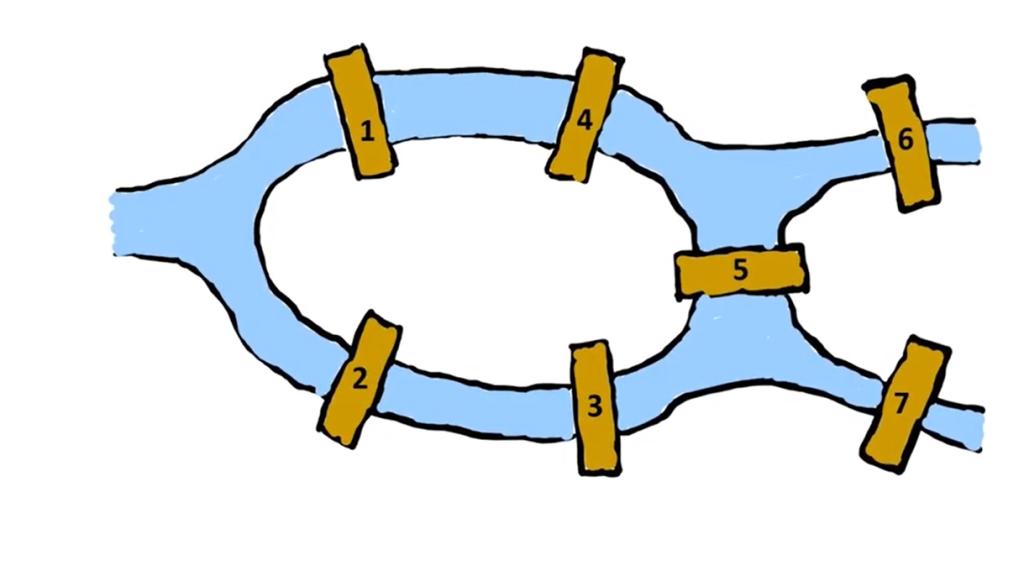
\includegraphics[scale=0.3]{Koningsberg_bridge_problem}
\end{figure}
Тут зображені всі острови та мости міста Кьонінгсберг (зараз поки Калінінград). Він намагався зрозуміти, чи можна обійти тільки один (!) раз всі мости, щоб повернутися до старту. Цю задачу можна звести в вигляді такого графу:
\begin{figure}[H]
\centering
\begin{tikzpicture}
\fill (0,0) circle (2pt) node[anchor = east] {$A$};
\fill (0,-2) circle (2pt) node[anchor = north east] {$D$};
\fill (0,2) circle (2pt) node[anchor = south east] {$C$};
\fill (3,0) circle (2pt) node[anchor = west] {$B$};

\draw plot [smooth, tension=2] coordinates {(0,0) (-0.3,-1) (0,-2)};
\draw plot [smooth, tension=2] coordinates {(0,0) (0.3,-1) (0,-2)};
\draw plot [smooth, tension=2] coordinates {(0,0) (-0.3,1) (0,2)};
\draw plot [smooth, tension=2] coordinates {(0,0) (0.3,1) (0,2)};
\draw (0,0)--(3,0);
\draw (0,-2)--(3,0);
\draw (0,2)--(3,0);
\end{tikzpicture}
\caption*{Кожній літері відповідає острів на малюну вище.}
\end{figure}
Насправді, виявляється, ми не зможемо обійти кожний міст один раз, щоб повернутися до старту. Відповідь на це дає наступна теорема:
\end{remark}

\begin{theorem}[Теорема Ойлера]
Зв'язний граф -- ойлерів $\iff$ всі вершини парні.
\end{theorem}

\begin{proof}
\rightproof Дано: зв'язний граф -- ойлеровий. Тобто існує ойлерів цикл, який, у свою чергу, містить всі ребра графу без повторень. Нехай якась вершина $v$ міститься $k$ разів у циклі (допускається, що до вершини можемо кілька разів повернутися). Звідси в циклі будуть такі частинки шляха: $e_{n_1-1}ve_{n_1}$,\ $e_{n_2-1}v e_{n_2}$, \dots , $e_{n_k-1}ve_{n_k}$. Всі ці ребра різні. Можна зауважити, що тут $2k$ ребер, що інцидентні вершині $v$. Звідси $d_v = 2k$ -- парне. І так з будь-якою іншою вершиною.\\
Для початкової вершини $v_0$ аналогічно як з $v$ буде $2k$ ребер, але ще плюс два ребра -- це стартове ребро та кінцеве ребро.
\bigskip \\
%Constructive proof
\iffalse
\leftproof Дано: зв'язний граф, де всі вершини -- парні (припускається, що граф непорожній).\\
Зафіксуємо довільну вершину $v_0 \in V$. Починаючи з неї, будуємо цикл, який містить без повторень деякі (не обов'язково всі) ребра графу $G$. Оскільки граф зв'язний, то існує ребро $e_1$, що інциентне $v_0$. Ребро $e_1$ веде від $v_0$ до деякої іншої вершини $v_1 \neq v_0$. Оскільки $v_1$ парна, то існує принаймні одне ребро $e_2 \neq e_1$, інцидентне вершині $v_1$.\\
Загалом нехай на $n$-му кроці побудовано шлях $v_0e_1v_1\dots e_nv_n$, причому $v_k \neq v_0, 0 < k < n$ та всі ребра різні (вершини не обов'язково різні). Якщо $v_n = v_0$, то маємо цикл.\
Інакше $v_n \neq v_0$, нехай $v_n$ входить у побудований шлях $m$ разів. Тоді всього $2m-1$ ребер, інцидентних $v_n$. Отже, має існувати хоча б одне ребро $e_{n+1}$, що інцидентне $v_n$ та не входить у побудований шлях (просто тому що $v_n$ -- парна вершина). І т.д. Цей процес закінчиться рано чи пізно, бо кількість ребер -- скінченна.
\bigskip \\
Нехай цикл $P$, що побудований був на абзаці вище, містить не всі ребра (у протилежному випадку цикл був би ойлеровим). Розглянемо підграф, де ми видалили всі ребра, що увійшли в $P$. Кожна вершина підграфу -- все одно всі вершини будуть парними (?). Але початковий граф -- зв'язний, тоді $P$ містить принаймні одну вершину $v_k$, що інцидентна деякому ребру підграфу. А далі побудуємо цикл, стартанувши з $v_k$ для підграфу, як це було на першому абзаці. Отримаємо цикл $Q$, що містить без повторень деякі (але, можливо, досі не всі) ребра підграфу.\\
Побудуємо цикл $P_1 = v_k P v_k Q v_k$, що містить без повторень всі ребра з $P,Q$. Далі повторюємо для $P_1$ ту же процедуру. І т.д. Цей процес закінчиться рано чи пізно.\\
У результаті, якийсь $P_n$ буде побудованим ойлеровим циклом.
\fi

%Alternative proof by the way of contradictions
\leftproof Дано: зв'язний граф $G$, де всі вершини -- парні (припускається, що граф непорожній).\\
Нехай $T$ -- деякий шлях графа $G$, що має максимальну довжину, де ребра не повторюються. Інтуїтивно дивлячись на ойлерові графи, ми очікуємо, що $T$ буде не просто шляхом, а ще й циклом.\\
!Припустимо, що $T$ -- не цикл, тобто $v_{\text{start}} \neq v_{\text{end}}$. Обчислимо степінь вершини $v_{\text{end}}$. Уже є одне ребро кінцеве, що йому інцидентне. Але всередині шляху цей $v_{\text{end}}$ може міститися $k$ разів -- у результаті, ми отримаємо ще $2k$ інцидентних ребер. Отже, $d_{v_{\text{end}}} = 2k+1$. Проте, за умовою, $d_{v_{\text{end}}}$ має бути парним числом. Тож знайдеться ще одне ребро (що не потрапило в $T$), яке інцидентне $v_{\text{end}}$, і ми рухаємось до вершини $w$ (ця вершина може потрапити в $T$). Але тоді ми знайшли ще більший шлях -- суперечність!\\
Значить, $T$ -- обов'язково цикл. Позначимо його за $C$. Залишилося переконатися, що цикл містить усі ребра.\\
!Припустимо, що $C$ не містить усі ребра. Тож існує ребро $\tilde{e}$, яка не міститься в $C$. Але має існувати $v \in C$, з якої стартуємо, та, проходячи по $\tilde{e}$, ми потрапимо в іншу якусь вершину $x \notin C$ (в силу зв'язності графа). А далі будуємо шлях $x \tilde{e} v C v$ -- отримали більший шлях за $C$ -- суперечність!\\
Висновок: $C$ -- цикл, що містить всі різні ребра. Тож граф -- ойлерів.
\end{proof}

\iffalse
%Remark for constructive proof
\begin{remark}
Мабуть, варто детально розібрати (?).\\
Маємо граф $G = (V,E)$ -- зв'язний, де вершини -- всі парні. Ми вже побудували цикл $v_0 e_1 v_1 e_2 v_2 \dots e_{n-1}v_{n-1} e_n v_0$, тут всі ребра різні (але не всі взяті з множини $E$). Тепер ми створимо $G'$ шляхом видалення цих ребер. Для $v_0$ степінь зменшиться на одиницю після видалення $e_1$ та ще на одиницю після видалення $e_n$. Нехай $v \neq v_0$ в циклі був $m \geq 0$ разів, тоді там $2m$ інцидентних ребер. А значить, степінь зменшиться, але буде далі парним.
\end{remark}
\fi

\begin{example}
Зокрема розглянемо задачу з мостами Кьонінгсберга.\\
Зауважимо, що існує вершина $v_B$, для якої $d_{v_B} = 3$ -- непарне число. За теоремою Ойлера, даний граф більше не буде ойлеровим (тобто не існує ойлерового циклу).
\end{example}

\begin{corollary}
Зв'язний граф -- напівойлерів $\iff$ граф містить не більше, ніж дві непарні вершини.
\end{corollary}

\begin{proof}
\rightproof Дано: зв'язний граф -- напівойлерів. Тобто існує ойлерів шлях. З'єднаємо (тимчасово) початкові та кінцеві вершини. Тоді отримаємо ойлерів шлях, звідси всі вершини -- парні. Якщо видалити ребро, яке з'єднує початок та кінець, то тоді $d_{v_{\text{start}}}, d_{v_{\text{end}}}$, що були парними, стануть непарними.
\bigskip \\
\leftproof Дано: зв'язний граф має дві непарні вершини. З'єднаємо дві непарні вершини ребром -- всі вершини будуть парними. Тоді знайдеться ойлерів шлях. Але якщо видалити ребро, яке з'єднувало непарні вершини, отримаємо лише ойлерів шлях.
\end{proof}

\begin{example}
Зокрема розглянемо задачу з мостами Кьонінгсберга.\\
Маємо $d_{v_A} = 5,\ d_{v_B} = d_{v_C} = d_{v_D} = 3$ -- більше двох непарних вершин. Тобто даний граф не буде навіть напівойлеровим.
\end{example}

\begin{remark}
За наявності рівно двох непарних вершин у зв'язному графі ойлерів шлях має починатися та закінчуватися саме в непарних вершинах.
\end{remark}

\subsubsection*{Алгоритм Флюорі}
Даний алгоритм застосовується при побудові ойлерового циклу (шляху), якщо граф -- ойлерів (напівойлерів).
\bigskip \\
1. У напіойлеровому графі беремо будь-яку непарну вершину. У ойлерових графах беремо довільну вершину.\\
2. Під час побудови циклу (шляху) з графу видаляємо ребра, що входять до циклу (шляху).\\
3. На кожному кроці можна обрати будь-яке ребро, що (за можливістю) не є мостом; міст обираємо лише тоді, коли всі ребра, індицентні даній вершині, є мостами.\\
\textit{Без доведення.}

\begin{example}
Нехай задано ось такий граф:
\begin{figure}[H]
\centering
\begin{tikzpicture}
\fill (0,0) circle (1pt) node[anchor = east] {$v_1$};
\fill (1,0.5) circle (1pt) node[anchor = south] {$v_2$};
\fill (2,0) circle (1pt) node[anchor = west] {$v_3$};
\fill (0,-2) circle (1pt) node[anchor = north] {$v_4$};
\fill (2,-2) circle (1pt) node[anchor = north] {$v_5$};

\draw (0,0)--(0,-2) node at (-0.4,-1) {$e_1$};
\draw (0,0)--(1,0.5) node at (0.5,0.5) {$e_2$};
\draw (1,0.5)--(2,0) node at (1.5,0.5) {$e_3$};
\draw (2,0)--(2,-2) node at (2.4,-1) {$e_4$};
\draw (0,0)--(2,-2) node at (0.5,-0.8) {$e_5$};
\draw (0,0)--(2,0) node at (1,0.2) {$e_6$};
\draw (2,0)--(0,-2) node at (1.7,-0.8) {$e_7$};
\draw (2,-2)--(0,-2) node at (1,-1.8) {$e_8$};
\end{tikzpicture}
\caption*{Граф -- напівойлерів, бо $v_4,v_5$ -- лише вони непарні.}
\end{figure}
Отже, беремо довільну непарну вершину -- це буде $v_4$. Жодне ребро не є мостом, тому можна обрати довільне ребро -- наприклад, $e_1$. Далі закреслюємо це ребро. Отримали вже $v_4e_1v_1$.
\begin{figure}[H]
\centering
\begin{tikzpicture}
\fill[red] (0,0) circle (1pt) node[anchor = east] {$v_1$};
\fill (1,0.5) circle (1pt) node[anchor = south] {$v_2$};
\fill (2,0) circle (1pt) node[anchor = west] {$v_3$};
\fill (0,-2) circle (1pt) node[anchor = north] {$v_4$};
\fill (2,-2) circle (1pt) node[anchor = north] {$v_5$};

\draw (0,0)--(1,0.5) node at (0.5,0.5) {$e_2$};
\draw (1,0.5)--(2,0) node at (1.5,0.5) {$e_3$};
\draw (2,0)--(2,-2) node at (2.4,-1) {$e_4$};
\draw (0,0)--(2,-2) node at (0.5,-0.8) {$e_5$};
\draw (0,0)--(2,0) node at (1,0.2) {$e_6$};
\draw (2,0)--(0,-2) node at (1.7,-0.8) {$e_7$};
\draw (2,-2)--(0,-2) node at (1,-1.8) {$e_8$};
\end{tikzpicture}
\caption*{Червона точка -- це те, де ми зараз.}
\end{figure}
Знову із $v_1$ жодне ребро -- не міст. Тому оберемо довільне ребро -- наприклад, $e_2$. Знову закреслюємо -- отримали вже $v_4e_1v_1e_2v_2$.
\begin{figure}[H]
\centering
\begin{tikzpicture}
\fill (0,0) circle (1pt) node[anchor = east] {$v_1$};
\fill[red] (1,0.5) circle (1pt) node[anchor = south] {$v_2$};
\fill (2,0) circle (1pt) node[anchor = west] {$v_3$};
\fill (0,-2) circle (1pt) node[anchor = north] {$v_4$};
\fill (2,-2) circle (1pt) node[anchor = north] {$v_5$};

\draw (1,0.5)--(2,0) node at (1.5,0.5) {$e_3$};
\draw (2,0)--(2,-2) node at (2.4,-1) {$e_4$};
\draw (0,0)--(2,-2) node at (0.5,-0.8) {$e_5$};
\draw (0,0)--(2,0) node at (1,0.2) {$e_6$};
\draw (2,0)--(0,-2) node at (1.7,-0.8) {$e_7$};
\draw (2,-2)--(0,-2) node at (1,-1.8) {$e_8$};
\end{tikzpicture}
\caption*{Червона точка -- це те, де ми зараз.}
\end{figure}
\vdots 
Якщо так продовжувати, то отримаємо такий напівойлерів шлях:\\
$v_4e_1v_1e_2v_2e_2e_3v_3e_4v_5e_5v_1e_6v_3e_7v_4e_8v_5$.\\
Важливо зауважити, що це не єдиний можливий напівойлерів шлях.
\end{example}

\end{document}

